\documentclass[a4paper,12pt]{article}
%-----------------------------------------------------------
\usepackage[top=20mm, bottom=6.4mm, left=30mm, right=30mm]{geometry}
\usepackage[utf8]{inputenc}
\usepackage[T1]{fontenc}
\usepackage{graphicx}
\usepackage[export]{adjustbox}
\usepackage{pdfpages}
\graphicspath{ {./images/} }
\usepackage{amsmath}
\usepackage{amsfonts}
\usepackage{amssymb}
\usepackage{float}
\usepackage{listings}
\usepackage[version=4]{mhchem}
\usepackage{stmaryrd}
\usepackage{xcolor}
\usepackage{attachfile}
\usepackage{amssymb}
\usepackage{booktabs}
\usepackage{multirow}
\usepackage{subcaption}
\usepackage{natbib}
\usepackage{wrapfig}
% \usepackage{iitbieortitle}
\usepackage{fancyhdr} % Added package for header customization

\definecolor{codegreen}{rgb}{0,0.6,0}
\definecolor{codegray}{rgb}{0.5,0.5,0.5}
\definecolor{codepurple}{rgb}{0.58,0,0.82}
\definecolor{backcolour}{rgb}{0.95,0.95,0.92}

\lstdefinestyle{mystyle}{
    backgroundcolor=\color{backcolour},   
    commentstyle=\color{codegreen},
    keywordstyle=\color{magenta},
    numberstyle=\tiny\color{codegray},
    stringstyle=\color{codepurple},
    basicstyle=\ttfamily\footnotesize,
    breakatwhitespace=false,         
    breaklines=true,                 
    captionpos=b,                    
    keepspaces=true,                 
    numbers=left,                    
    numbersep=5pt,                  
    showspaces=false,                
    showstringspaces=false,
    showtabs=false,                  
    tabsize=2
}

\lstset{style=mystyle}

% Define header and footer
\pagestyle{fancy}
\fancyhf{} % Clear header and footer
\rhead{\thepage} % Right-aligned page number in the header
\lhead{\textit{\title}} % Left-aligned title in the header

\begin{document}
\lstset{language=Matlab,%
    %basicstyle=\color{red},
    breaklines=true,%
    morekeywords={matlab2tikz},
    keywordstyle=\color{blue},%
    morekeywords=[2]{1}, keywordstyle=[2]{\color{black}},
    identifierstyle=\color{black},%
    stringstyle=\color{mylilas},
    commentstyle=\color{mygreen},%
    showstringspaces=false,%without this there will be a symbol in the places where there is a space
    numbers=left,%
    numberstyle={\tiny \color{black}},% size of the numbers
    numbersep=9pt, % this defines how far the numbers are from the text
    emph=[1]{for,end,break},emphstyle=[1]\color{red}, %some words to emphasise
    %emph=[2]{word1,word2}, emphstyle=[2]{style},    
}



\begin{center}
    


\includegraphics[max width = \textwidth]{iitb_logo.png}
    
    {\it{\Large{I}\large{NDIAN} \Large{I}\large{NSTITUTE OF} \Large{T}\large{ECHNOLOGY,} \Large{B}\large{OMBAY}}}\\
    \vspace{3em}
    
    \huge{MIXED} \huge{SIGNAL} \huge{VLSI DESIGN}\\
    \vspace{0.5em}

    \Large{EE - 719}\\
    \vspace{2em}
    
    \hline
    \vspace{0.5em}
    
    \textbf{\huge{9-Bit Hybrid Fully Differential ADC }}\\
    % \textbf{\huge{GCD calculation using VHDL}}
    \vspace{0.5em}
    
    \hline\\
    
    \vspace{2em}

    Name : \hfill{Roll Number :}\\
    Abhijeet \hfill{20D070003}\\
    G Kamalesh \hfill{20D070029}\\

    \vspace{1em}
    Professor : \hfill{Maryam Shojaei Baghini}\\
    

    \vspace{2em}

   Feb. 20, 2023
    

    
\end{center}

\newpage

\section{Bootstrap Switch Design}
\begin{figure}[H]
    \centering
    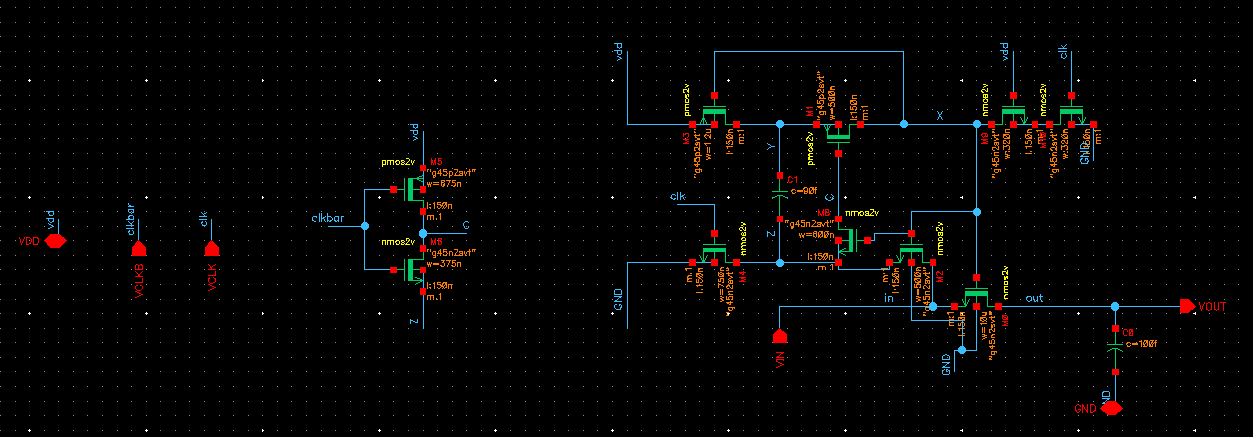
\includegraphics[scale=0.5]{Images/bootstrap_sch.png}
    \caption{Bootstrap Switch Schematic}
    \label{fig:enter-label}
\end{figure}

\begin{figure}[H]
    \centering
    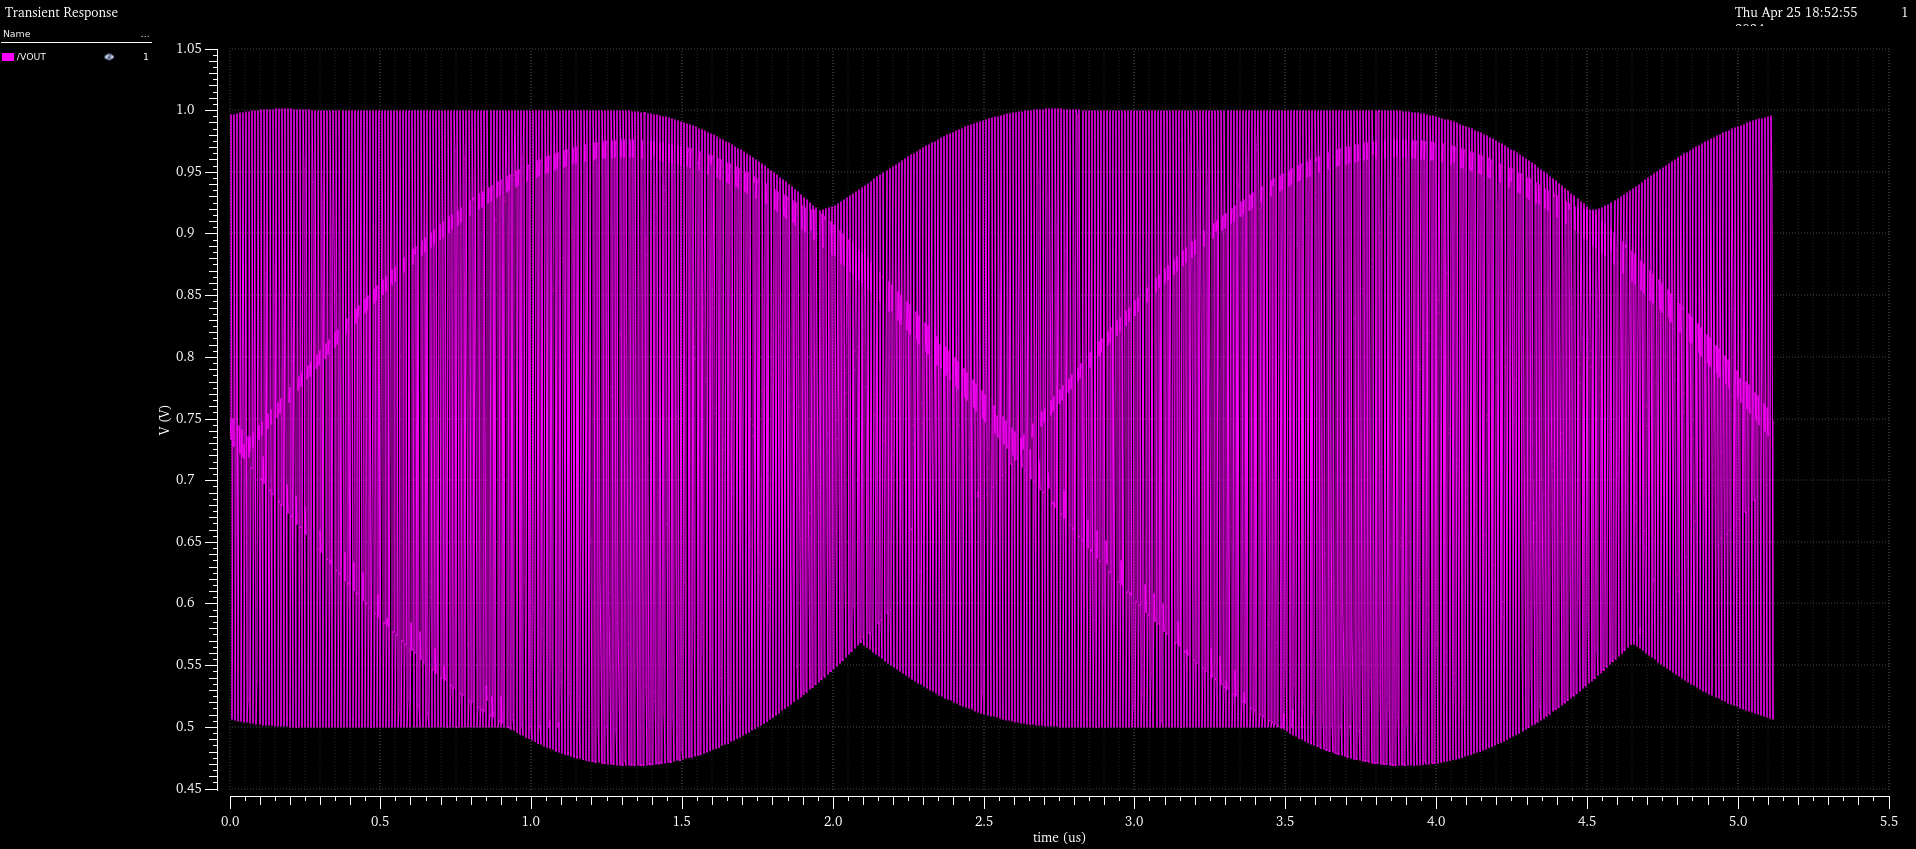
\includegraphics[max width = \textwidth]{Images/bootstrap_out.png}
    \caption{Bootstrap output waveform}
    \label{fig:enter-label}
\end{figure}

\begin{figure}[H]
    \centering
    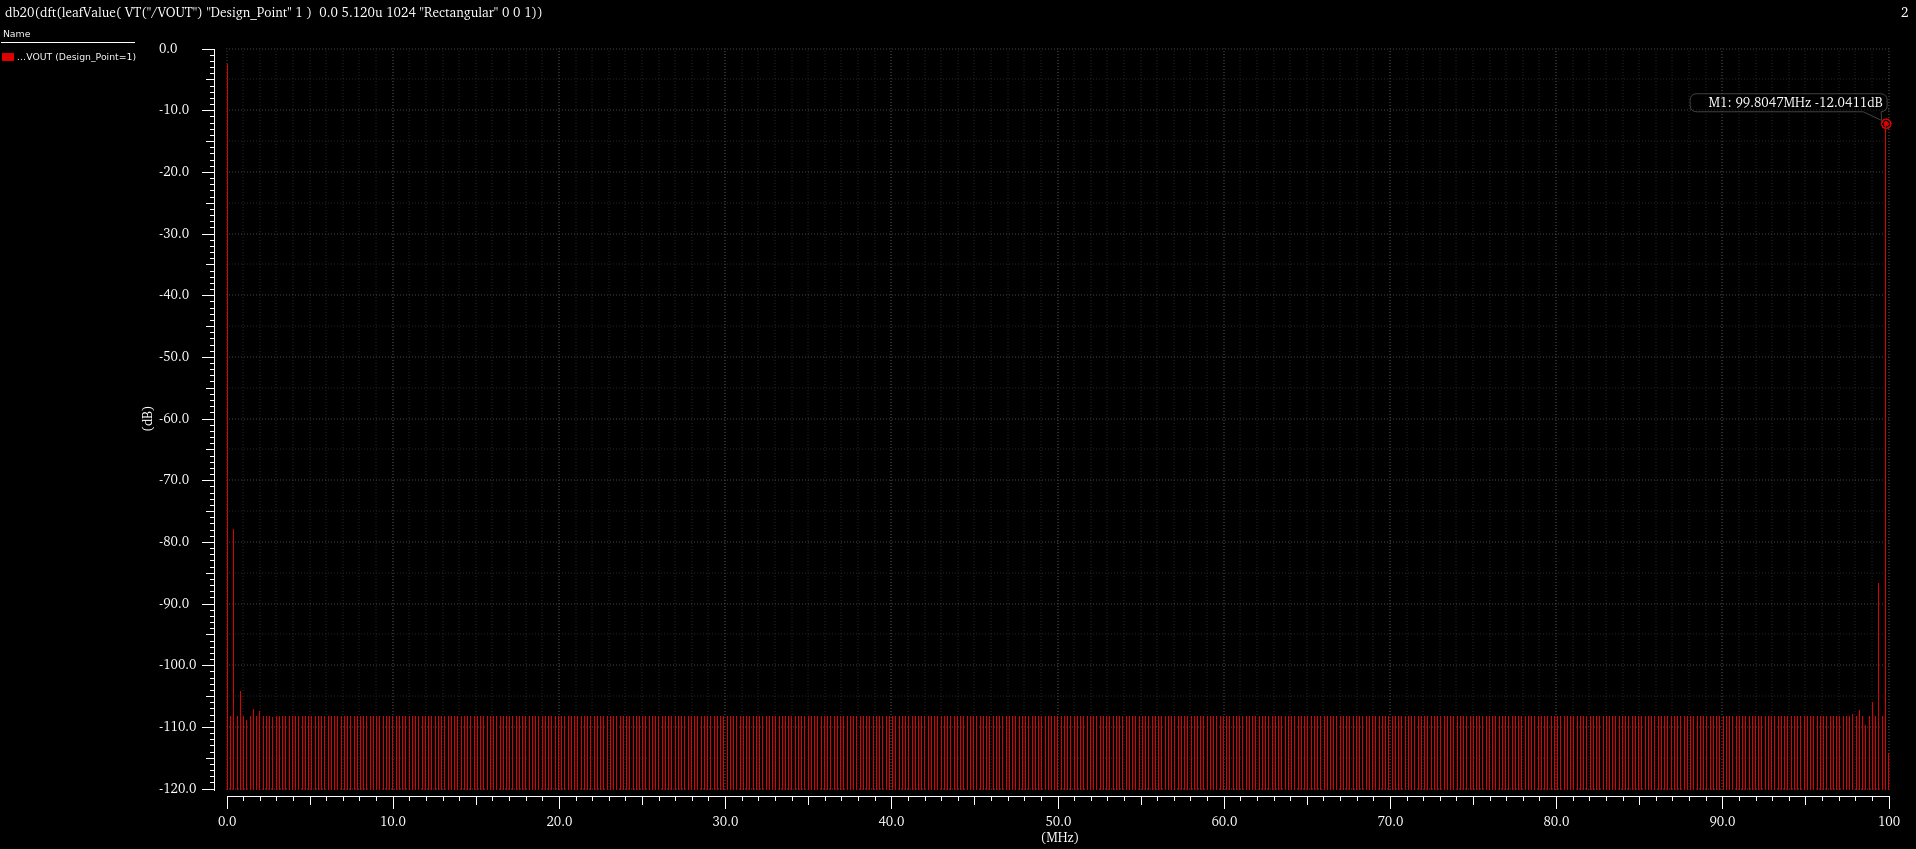
\includegraphics[max width = \textwidth]{Images/bootstrap_out_fft.png}
    \caption{FFT of Bootstrap output waveform}
    \label{fig:enter-label}
\end{figure}

This 9 bit bootstrap switch is giving ENOB 10.28.

\begin{figure}[H]
    \centering
    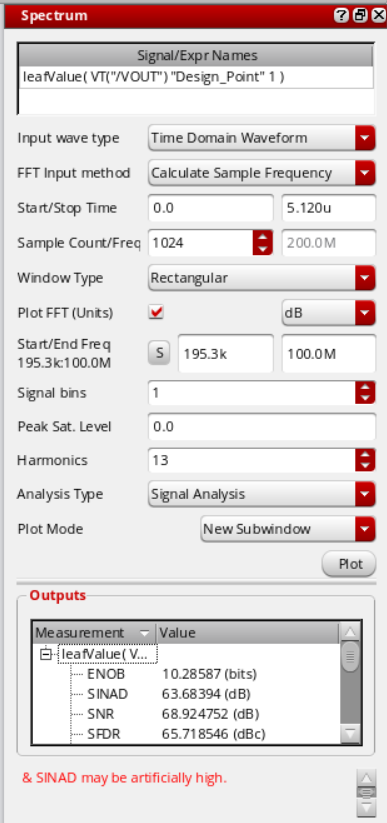
\includegraphics[max width = \textwidth]{Flash_ADC_images/Bootstrap_SNR.png}
    \caption{Bootstrap SNR}
    \label{fig:enter-label}
\end{figure}

\textbf{[1.1] Report the final value of the widths and lengths of all transistors.}
\begin{table}[H]
    % \centering
    \begin{tabular}{|c|c|c|c|c|c|c|c|c|c|c|c|c|}
    \hline
       Parameter & $M_1$ & $M_2$ & $M_3$ & $M_4$ & $M_5$ & $M_6$ & $M_8$ & $M_a$  & $M_b$ & $M_c$ & C_1 & C_B \\
       \hline
        W(in m) & 10 $\mu$ & 500n & 500n & 320n$ & 1.2 $\mu$ & 750n & 320n & 675n & 375n & 600n & 90 fF & 100 fF\\
        \hline
        L(in nm) & 150 & 150  & 150  & 150  & 150  & 150  & 150  & 150  & 150  & 150 & X & X \\
        \hline
    \end{tabular}
    \caption{Final Parameter Summary of Bootstrap Switch}
    \label{tab:my_label}
\end{table}

\newpage

\section{3-bit differential Flash ADC Design}
\subsection{Preamplifier design}
The preamplifier is a fully differential amplifier designed to produce a gain of 2 before the comparator
\begin{figure}[H]
    \centering
    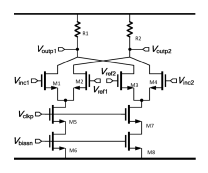
\includegraphics[max width = \textwidth]{Images/Preamp_circ.png}
    \caption{FFT of Bootstrap output waveform}
    \label{fig:enter-label}
\end{figure}
\begin{itemize}
    \item As a starting point we assumed to flow  a 25 uA current in the tail part of the pre-amplifier.
    \item For that value of current we tried to find the initial value of the biased transistor such that it will come the saturation region.
    \item At the Width of 1um and bias voltage of 0.6V. the bottommost transistor is in saturation mode.
    \item Now we increasd the current by increasing widths and of the differential pair and the biased transistors. So that differential pired transistors will be in saturation mode.
    \item Now our final task is to increase the gain for the worst case more than 2.
    \item That we achieved be increasing the bias voltage from 0.6V to 0.8 V and slight increments in the widths of the transistor.
\end{itemize}

\textbf{Initial parameters}

\begin{table}[H]
    \centering
    \begin{tabular}{|c|c|c|c|c|c|c|c|c|c|c|}
        \hline
         Design Variable & $M_1$ & $M_2$ & $M_3$ & $M_4$ & $M_5$ & $M_6$ & $M_7$ & $M_8$ & $R_1$ & $R_2$  \\
         \hline
         Width & 5um & 5um & 5um & 5um & 1um & 1m & 1um & 1um & 1K$\Omega$ & 1K$\Omega$ \\  
         \hline
         Length (nm) & 150 & 150 & 150 & 150 & 150 & 150 & 150 & 150 & & \\ 
         \hline
    \end{tabular}
    \caption{Initial parameters for Preamplfier}
    \label{tab:my_label}
\end{table}

    \textbf{Final parameters}
    \begin{table}[H]
        \centering
        \begin{tabular}{|c|c|c|c|c|c|c|c|c|c|c|}
        \hline
         Design Variable & $M_1$ & $M_2$ & $M_3$ & $M_4$ & $M_5$ & $M_6$ & $M_7$ & $M_8$ & $R_1$ & $R_2$  \\
         \hline
         Width & 40u & 40u & 20u & 20u & 10u & 10u & 10u & 10u & - & -\\
         \hline
         Length & 150n & 150n & 150n & 150n & 150n & 150n & 150n  & 150n & 1k & 1k\\
         \hline
        \end{tabular}
        \caption{Final parameters for Preamplifier}
        \label{tab:my_label}
    \end{table}
    \textbf{Please note that the transistor numberings are reversed in the table and the schematic}

\begin{figure}[H]
    \centering
    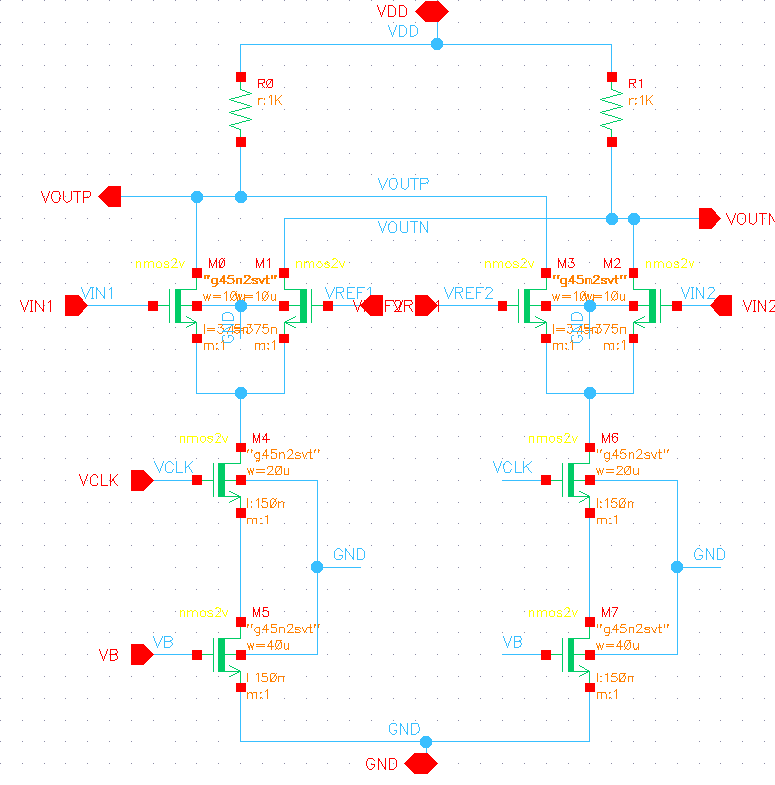
\includegraphics[max width = \textwidth]{Flash_ADC_images/Preamp_sch.png}
    \caption{Preamplifier schematic}
    \label{fig:enter-label}
\end{figure}

\subsection{Testing of Preamplifier}
\begin{itemize}
    \item[1.] Take Vref1 = 0.9375 V and Vref2 = 0.5625 V (worst case reference inputs in the flash ADC) and Vinc1 = Vcm + 0.25 Sin(2πfint) and Vinc2 = Vcm − 0.25 Sin(2πfint) and plot the transient output for fin = 50 MHz.

\begin{figure}[H]
    \centering
    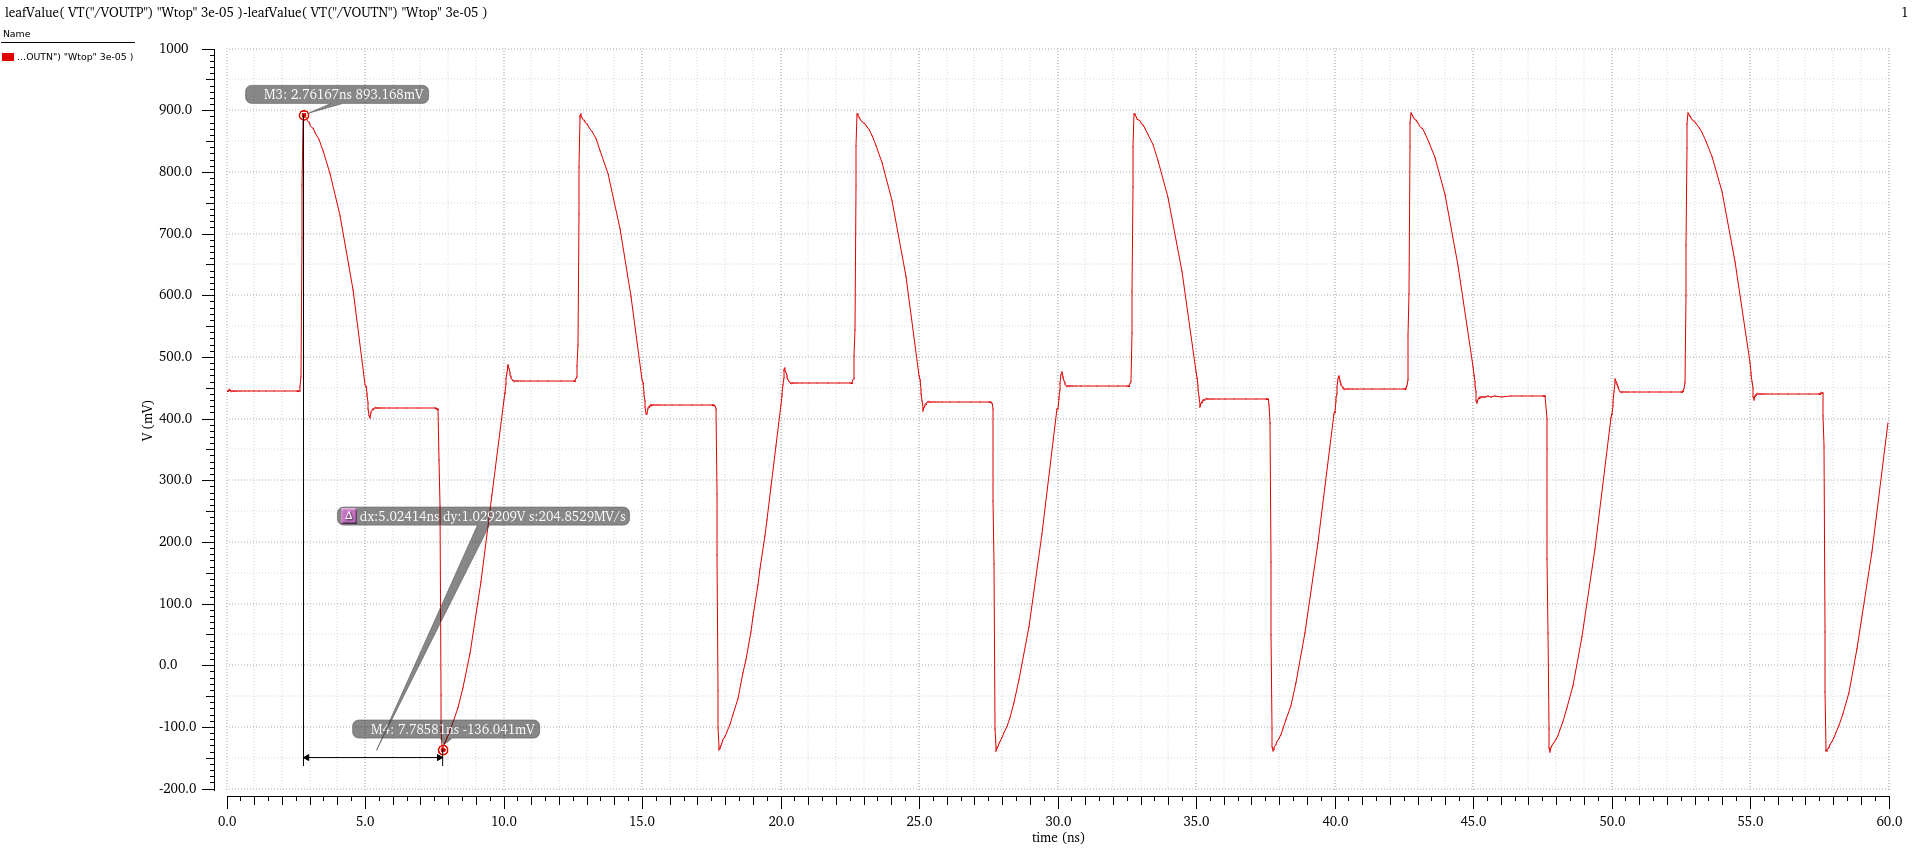
\includegraphics[max width = \textwidth]{Flash_ADC_images/Preamp_out.png}
    \caption{Preamplifier output waveform}
    \label{fig:enter-label}
\end{figure}

    \item[2.] Take Vref1 = 0.75 V and Vref2 = 0.75 V and Vinc1 = Vcm + 0.25 Sin(2πfint) and Vinc2 = Vcm − 0.25 Sin(2πfint) and plot the transient output for fin = 50 MHz.
    \begin{figure}[H]
    \centering
    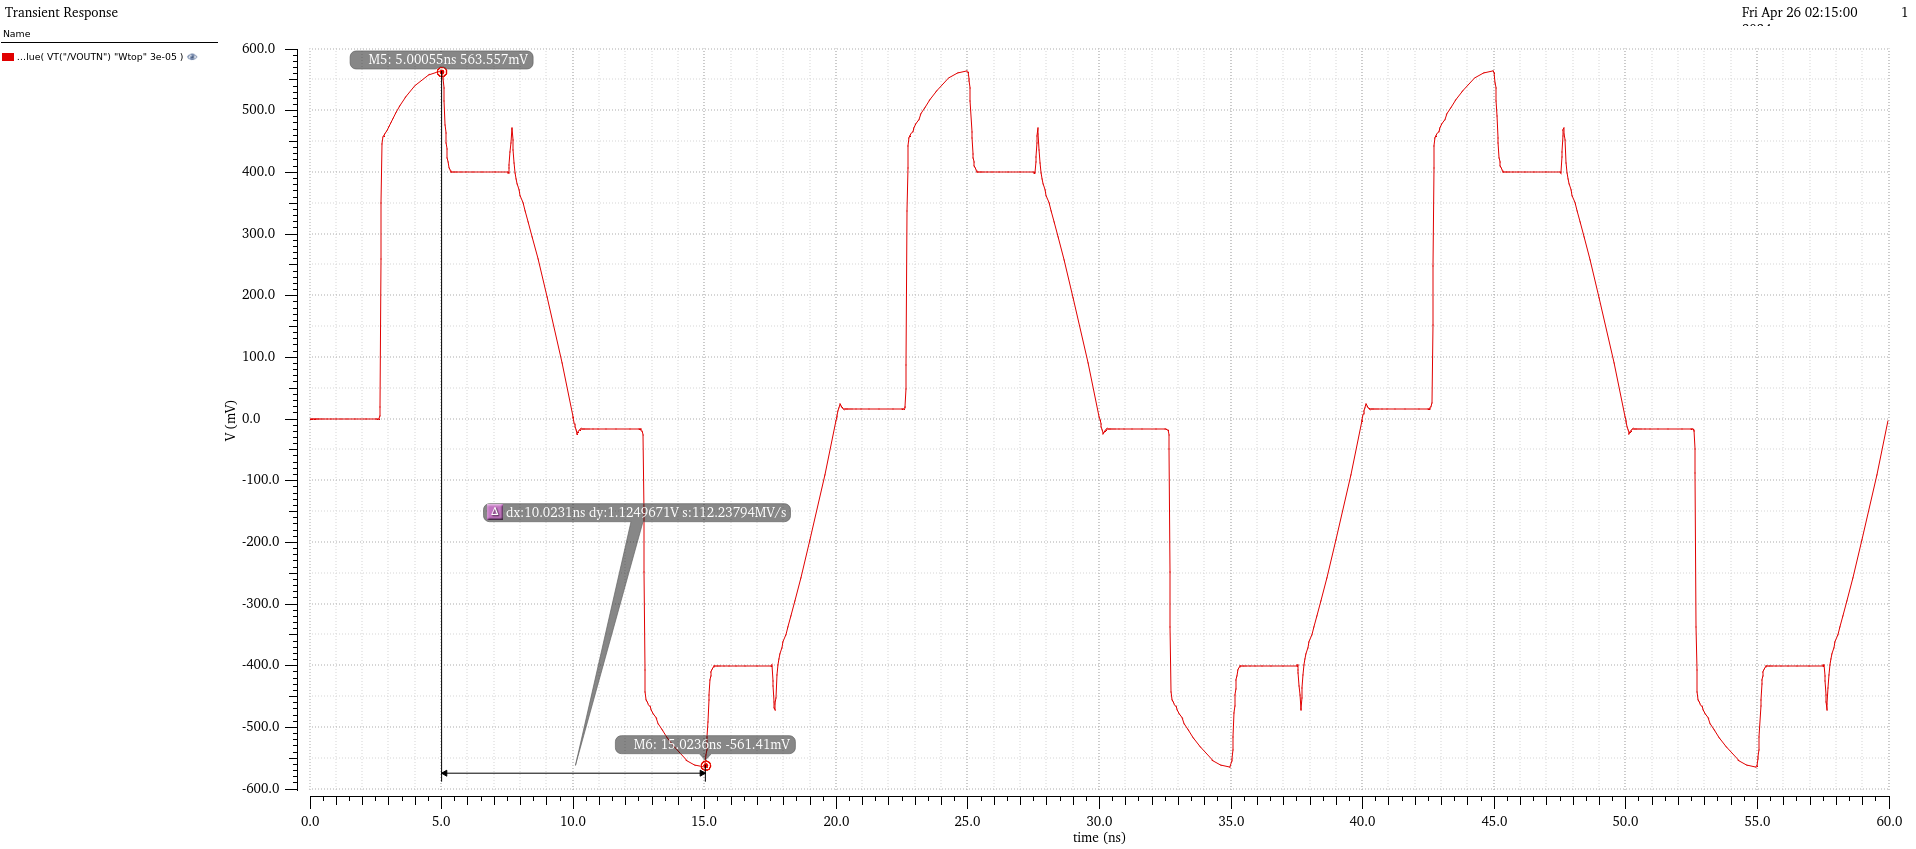
\includegraphics[max width = \textwidth]{Preamp_out_75ref.png}
    \caption{Preamplifier output waveform}
    \label{fig:enter-label}
\end{figure}

\subsection{Reuse of the comparator designed in assignment 5 + RS Latch}
\begin{figure}[H]
    \centering
    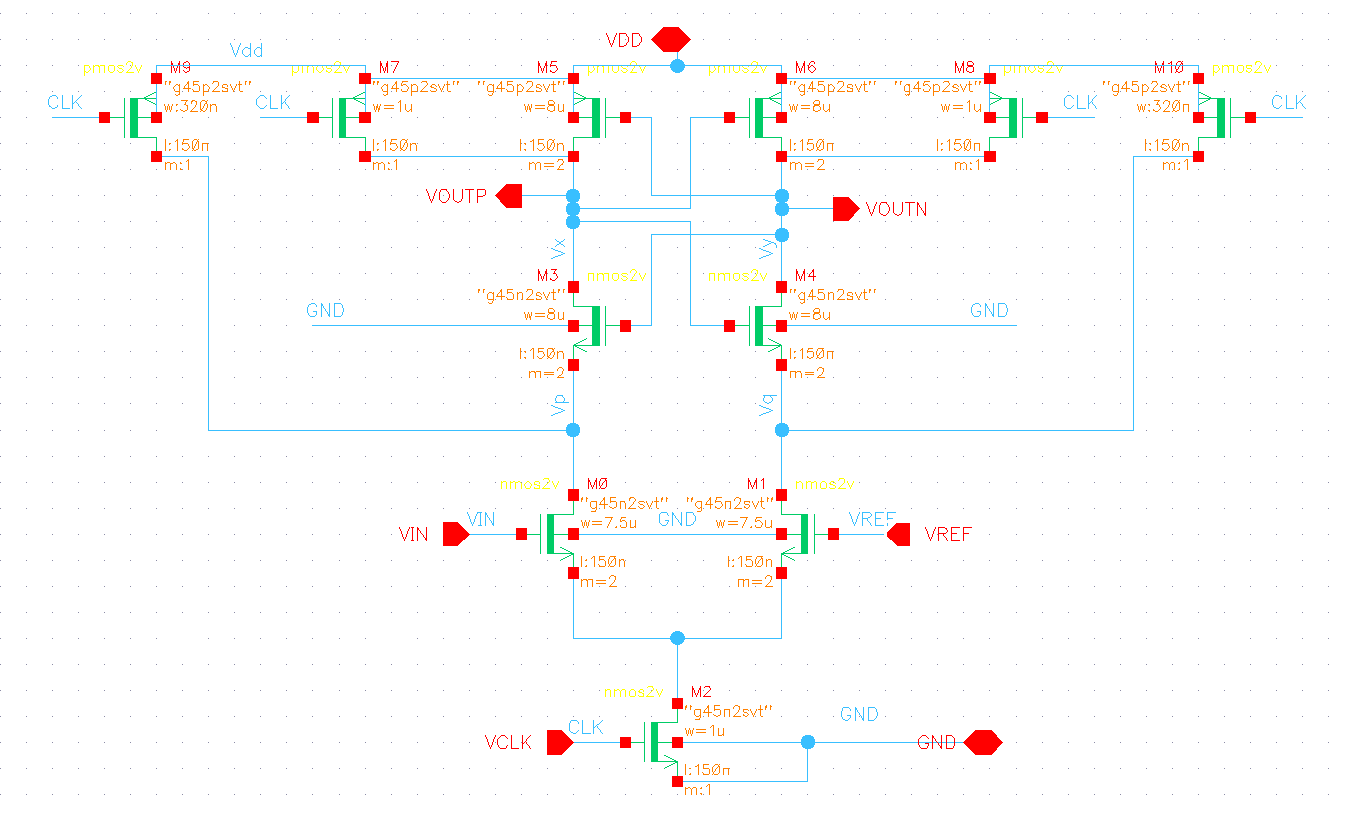
\includegraphics[max width = \textwidth]{Flash_ADC_images/SAL_sch.png}
    \caption{Strong arm Latch Comparator schematic}
    \label{fig:enter-label}
\end{figure}

\begin{figure}[H]
    \centering
    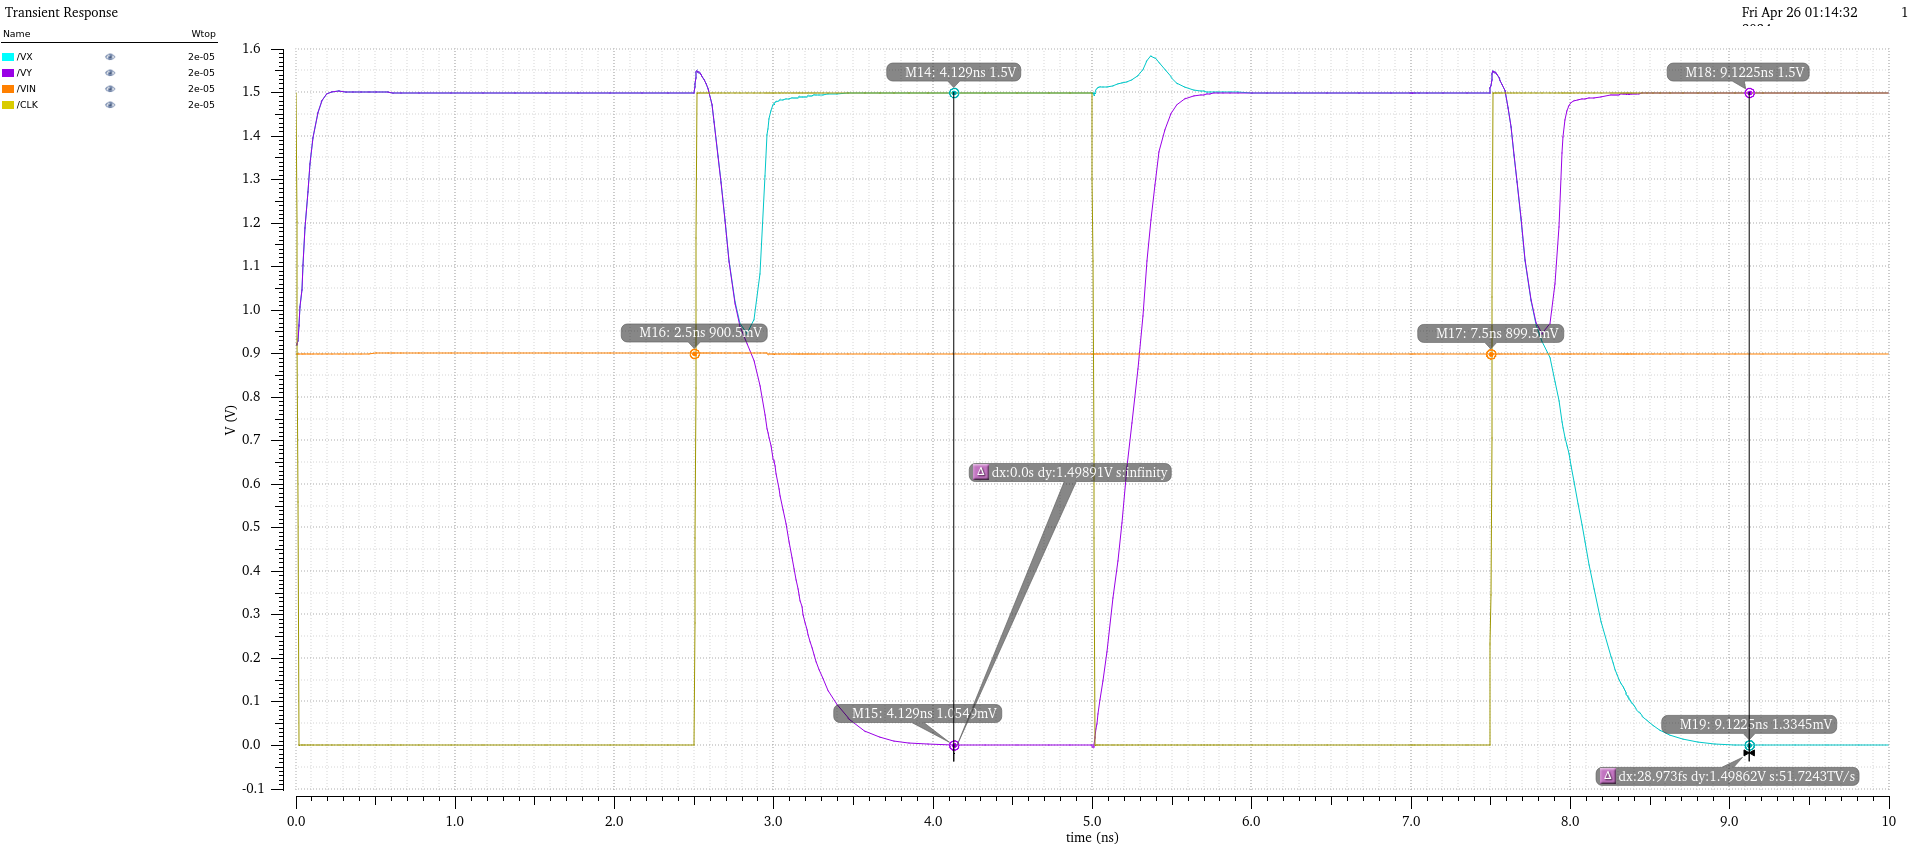
\includegraphics[max width = \textwidth]{Flash_ADC_images/SAL_out.png}
    \caption{Strong arm Latch Comparator schematic}
    \label{fig:enter-label}
\end{figure}

    \begin{table}[H]
        \centering
        \begin{tabular}{|c|c|c|c|c|c|c|c|c|}
        \hline
         Design Variable & $M_0$ & $M_1$ & $M_2$ & $M_3$ & $M_{P1}$ & $M_{N1}$ & $M_{P2}$ & $M_{N2}$ \\
         \hline
         Width & 5u & 5u & 10u & 10u & 640nmu & 320nm & 640nm & 320nm\\          
         \hline
         Length & 150n & 150n & 150n & 150n & 150n & 150n & 150n  & 150\\
         \hline
        \end{tabular}
        \caption{Initial parameters for Preamplifier}
        \label{tab:my_label}
    \end{table}

    \begin{table}[H]
        \centering
        \begin{tabular}{|c|c|c|c|c|c|c|c|c|}
        \hline
         Design Variable & $M_0$ & $M_1$ & $M_2$ & $M_3$ & $M_{P1}$ & $M_{N1}$ & $M_{P2}$ & $M_{N2}$ \\
         \hline
         Width & 20u & 20u & 25u & 25u & 640nm & 320nm & 640nm & 320nm\\          
         \hline
         Length & 150n & 150n & 150n & 150n & 150n & 150n & 150n  & 150\\
         \hline
        \end{tabular}
        \caption{Final parameters for Preamplifier}
        \label{tab:my_label}
    \end{table}

\begin{figure}[H]
    \centering
    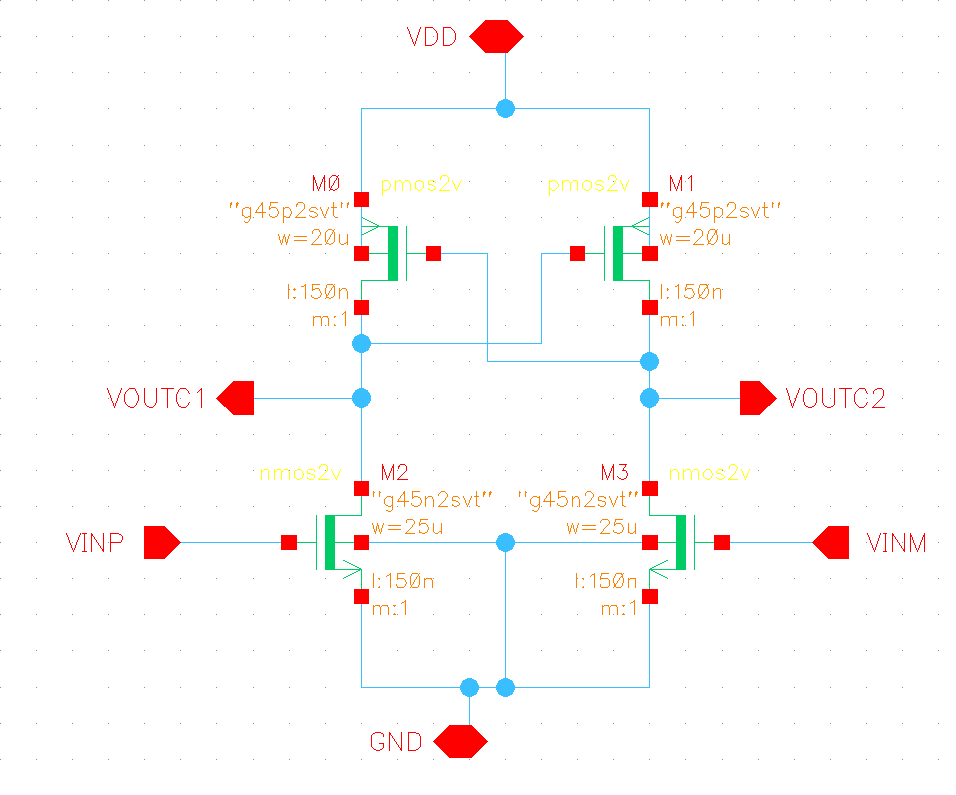
\includegraphics[max width = \textwidth]{Flash_ADC_images/RSLatch.png}
    \caption{RS Latch schematic}
    \label{fig:enter-label}
\end{figure}

\begin{figure}[H]
    \centering
    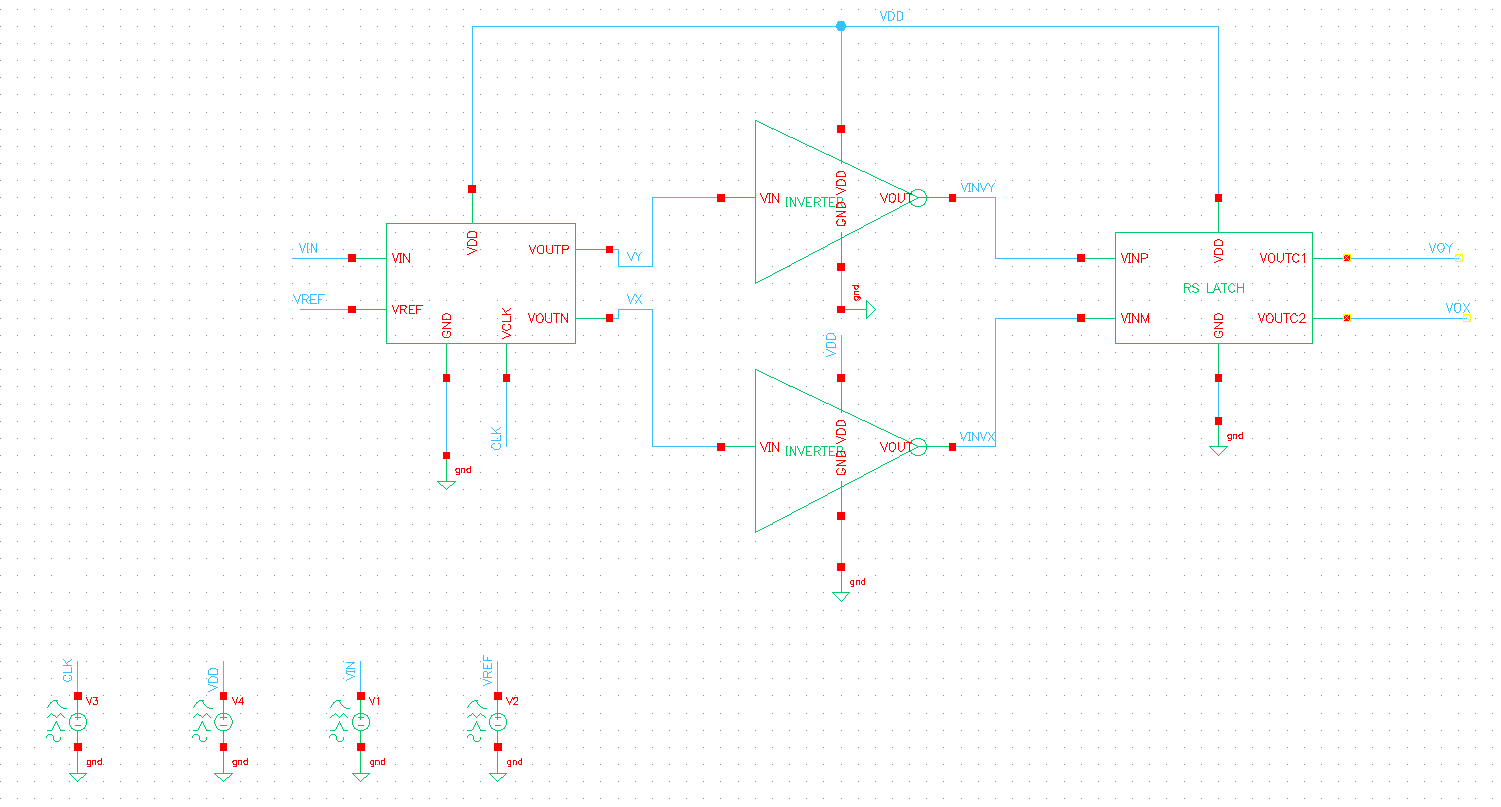
\includegraphics[max width = \textwidth]{Flash_ADC_images/SAL_RSLatch.png}
    \caption{Strong arm Latch Comparator followed by RS Latch Testbench}
    \label{fig:enter-label}
\end{figure}

\begin{figure}[H]
    \centering
    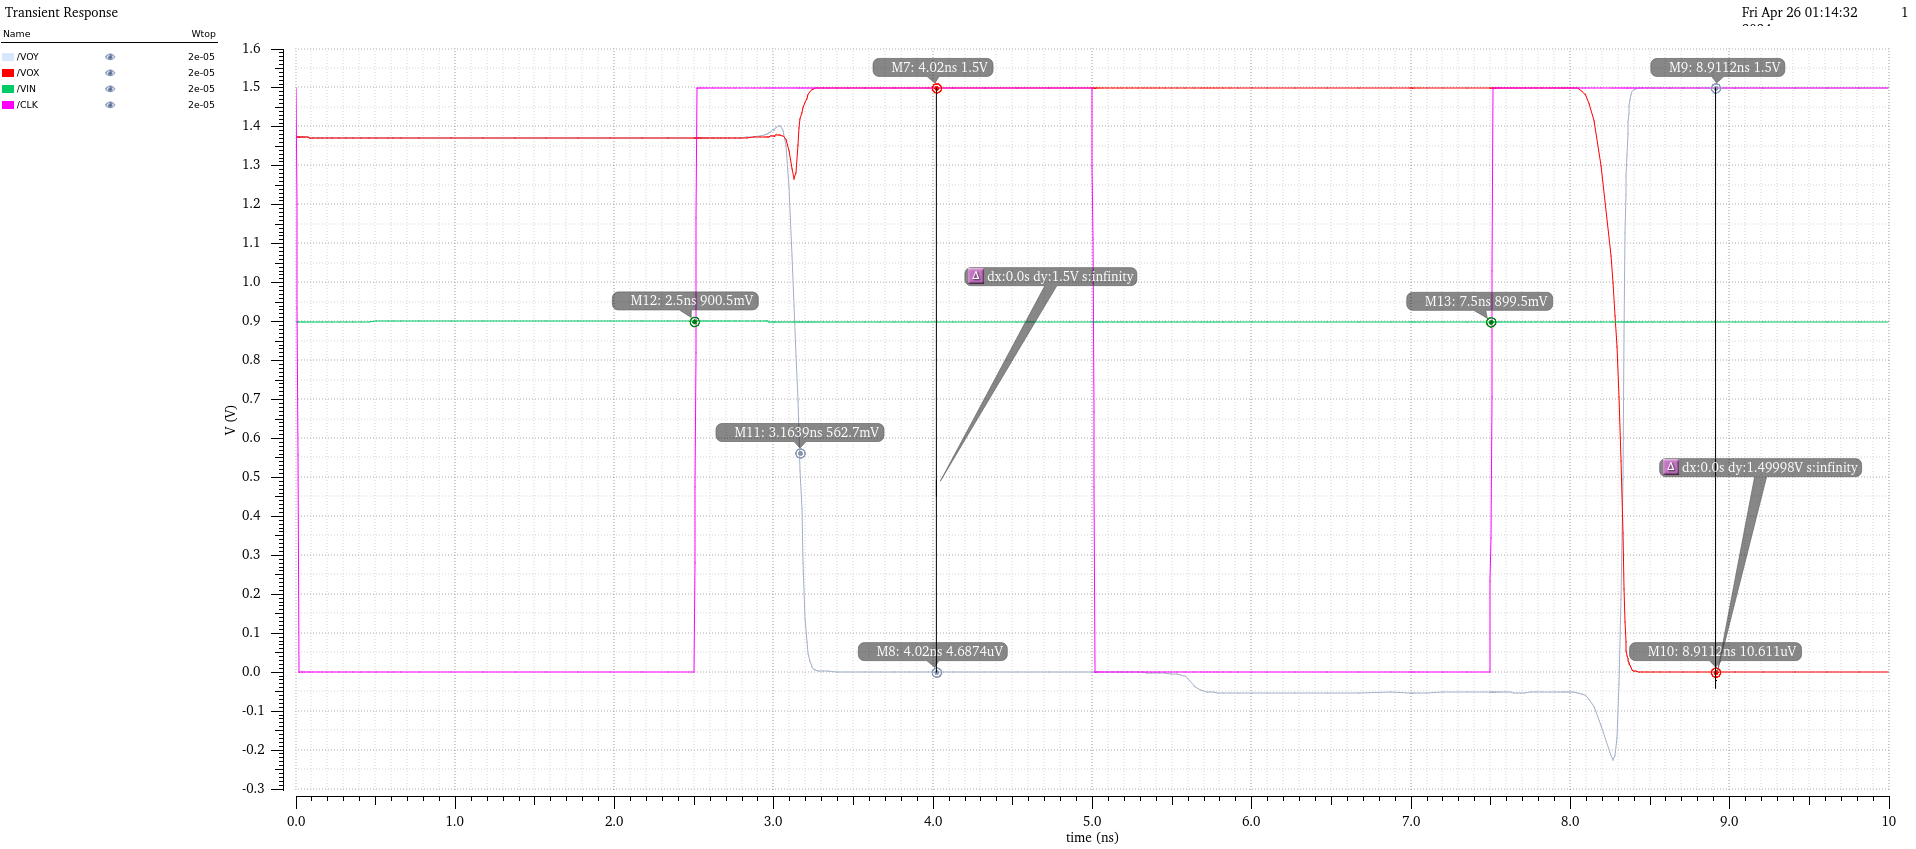
\includegraphics[max width = \textwidth]{Flash_ADC_images/RS_latch_out.png}
    \caption{Strong arm Latch followed by RS Latch output waveform}
    \label{fig:enter-label}
\end{figure}
\end{itemize}

\subsection{Differential Flash ADC}
\begin{figure}[H]
    \centering
    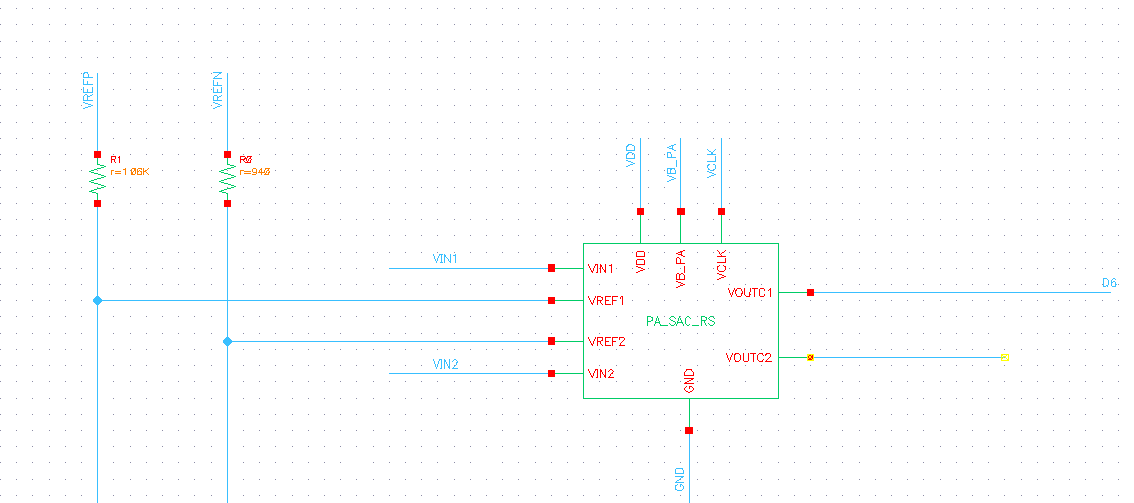
\includegraphics[max width = \textwidth]{Flash_ADC_images/temp_codegen.png}
    \caption{Temperature code generator}
    \label{fig:enter-label}
\end{figure}

\begin{figure}[H]
    \centering
    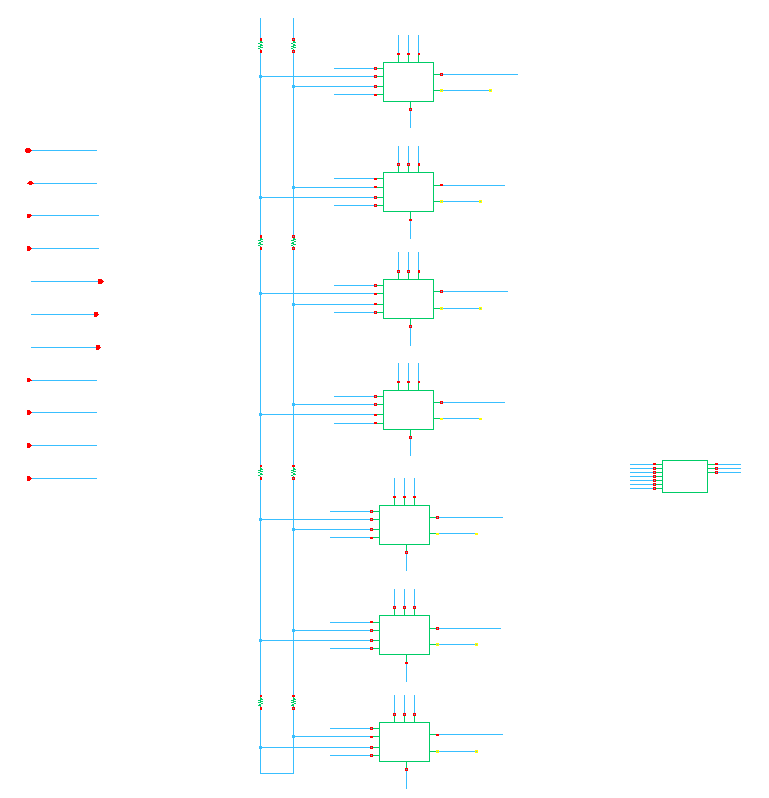
\includegraphics[max width = \textwidth]{Flash_ADC_images/flash_adc.png}
    \caption{3 Bit Fully differential Flash ADC}
    \label{fig:enter-label}
\end{figure}

\begin{figure}[H]
    \centering
    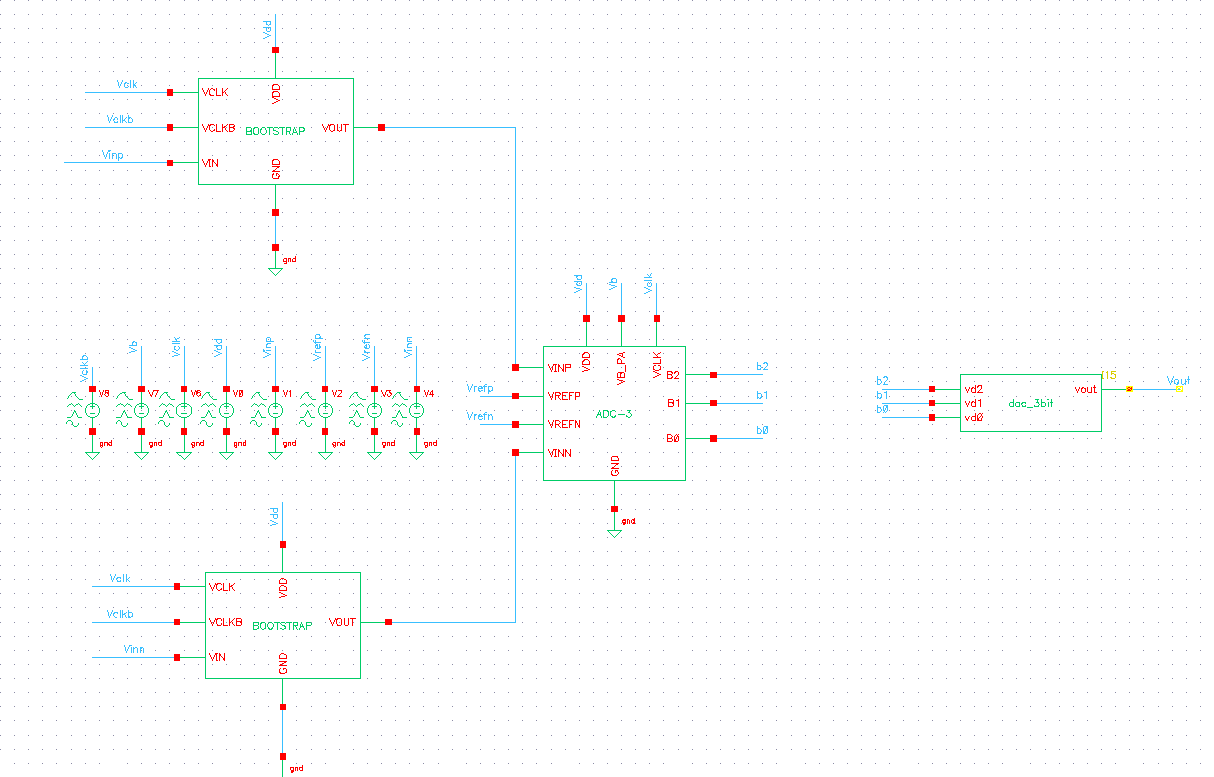
\includegraphics[max width = \textwidth]{Flash_ADC_images/flash_adc_test.png}
    \caption{Flash ADC Testbench}
    \label{fig:enter-label}
\end{figure}


\subsection{FFT with ADC + ideal DAC topology}

\begin{figure}[H]
    \centering
    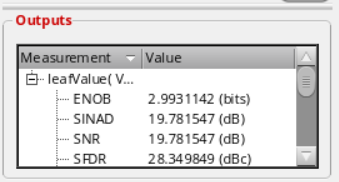
\includegraphics[width=1\linewidth]{flash_SNR.png}
    \caption{SNR of Flash ADC}
    \label{fig:enter-label}
\end{figure}

\begin{figure}[H]
    \centering
    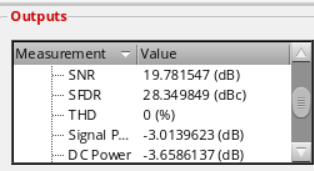
\includegraphics[width=1\linewidth]{flash_thd.png}
    \caption{THD of Flash ADC}
    \label{fig:enter-label}
\end{figure}
\subsection{INL DNL - non-linearities in the resistor}
The value of R is 1k $\Omega$ and hence, $\Delta$ R = 20 $\Omega$. The plots obtained by providing a ramp signal at the input are attached below:
\begin{figure}[H]
    \centering
    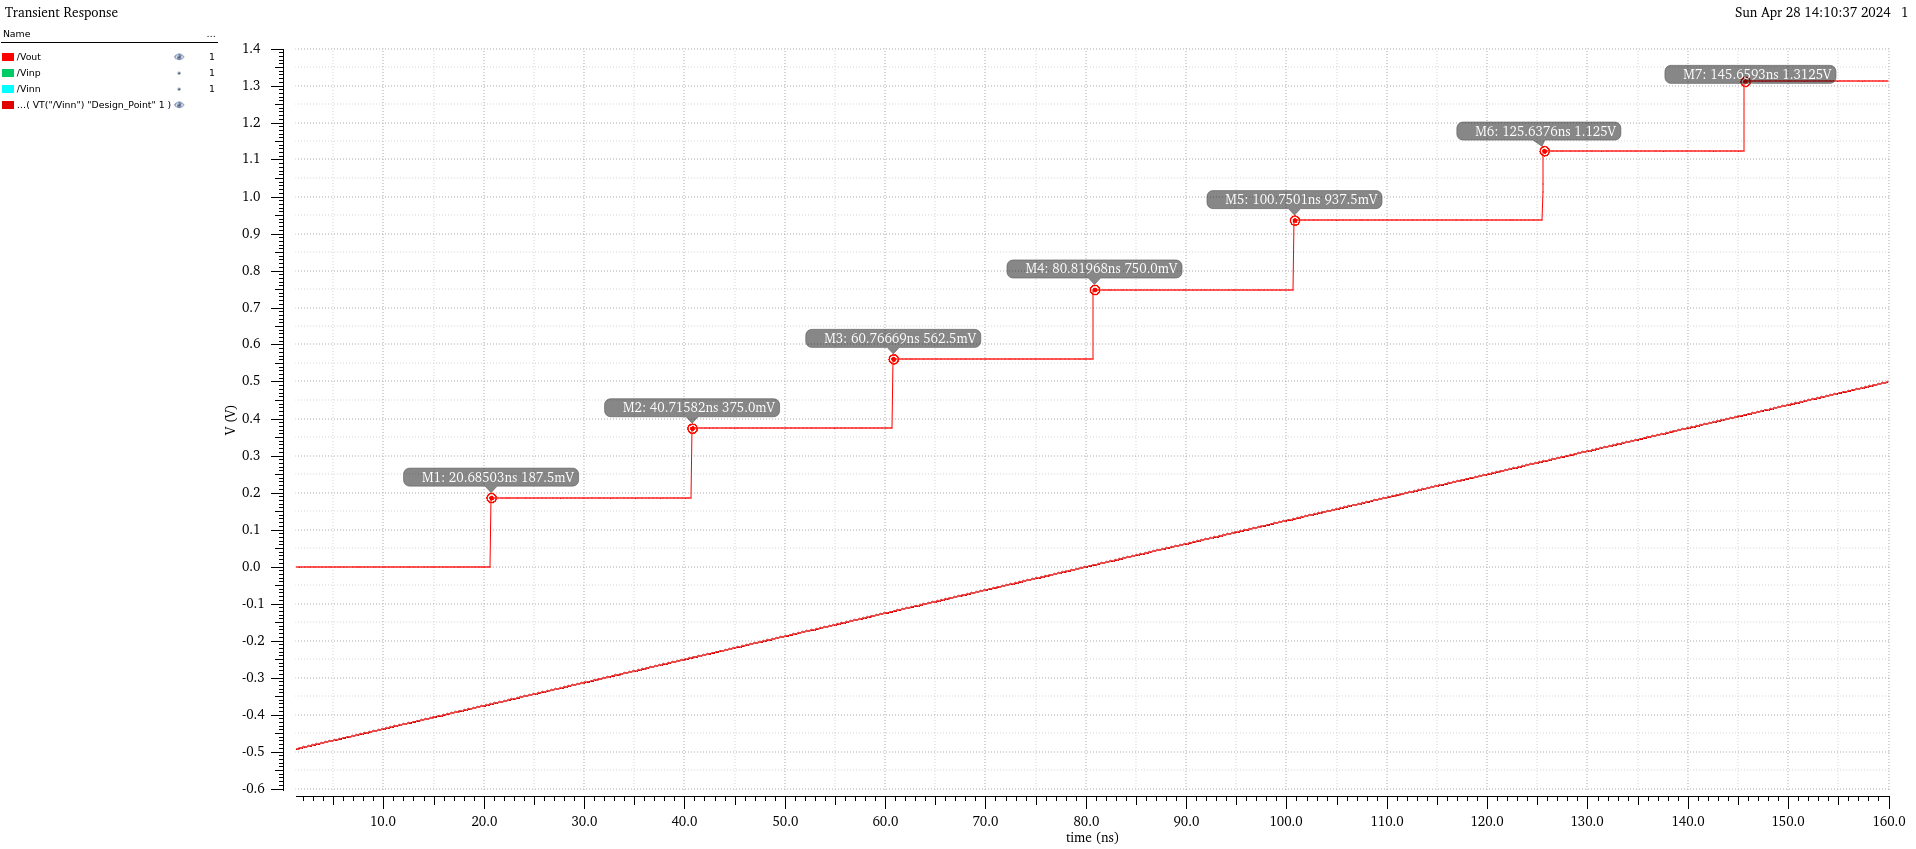
\includegraphics[max width = \textwidth]{Flash_ADC_images/INL_DNL_output.png}
    \caption{DAC Output vs Input characteristics}
    \label{fig:enter-label}
\end{figure}

\begin{figure}[H]
    \centering
    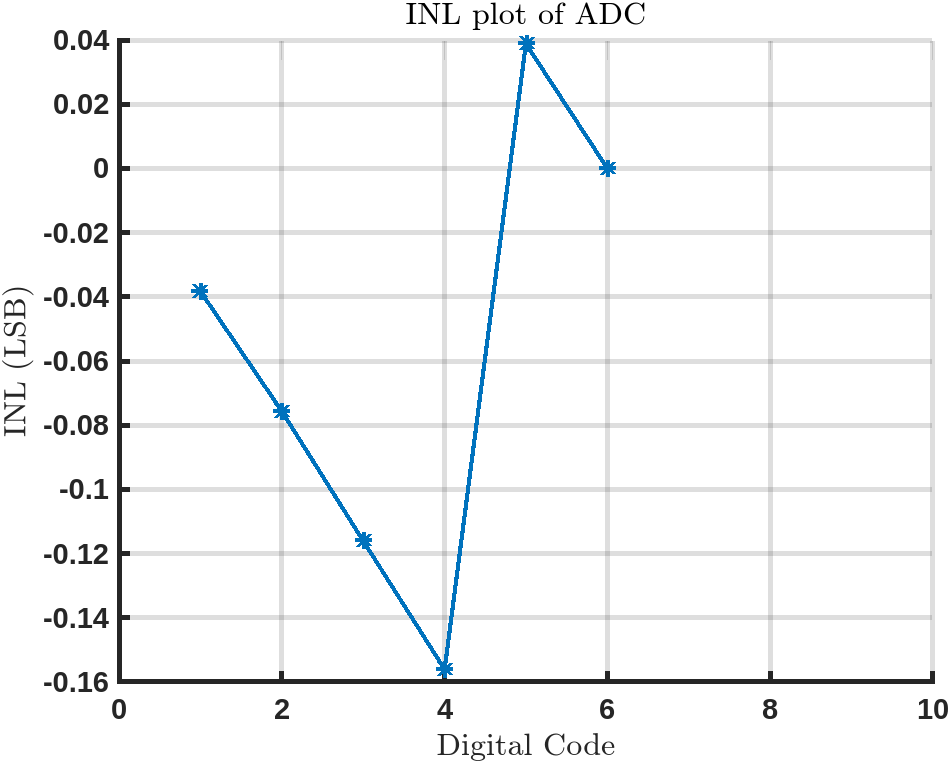
\includegraphics[max width = \textwidth]{Flash_ADC_images/INL.png}
    \caption{INL}
    \label{fig:enter-label}
\end{figure}

\begin{figure}[H]
    \centering
    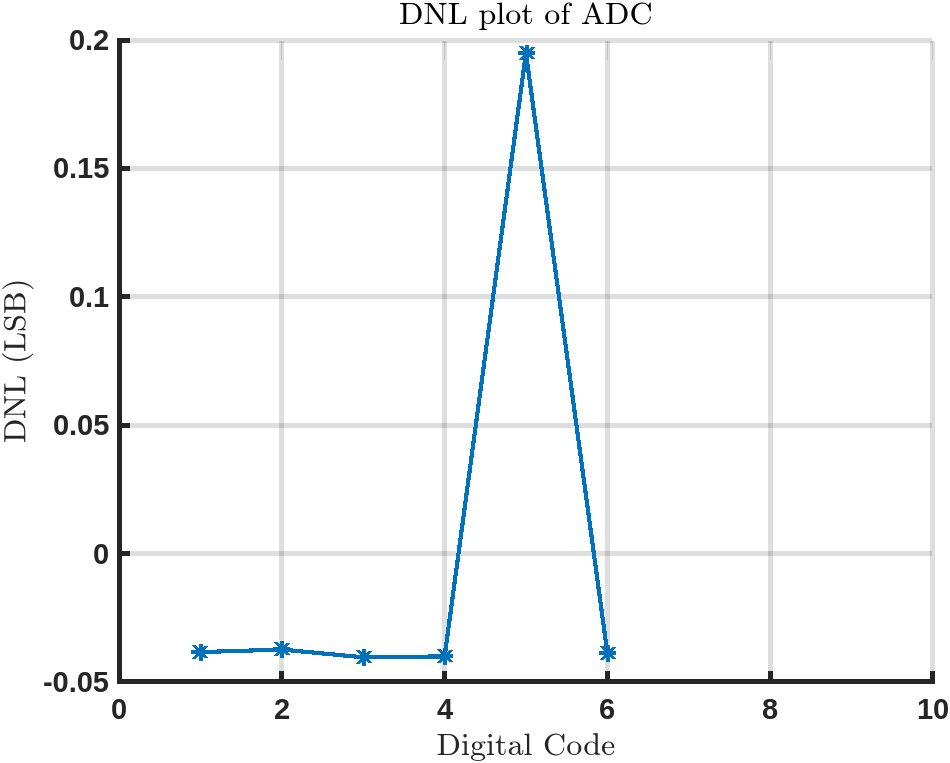
\includegraphics[max width = \textwidth]{Flash_ADC_images/DNL.png}
    \caption{DNL}
    \label{fig:enter-label}
\end{figure}

\section{Design of 6-bit Differential SAR ADC}
\begin{figure}
    \centering
    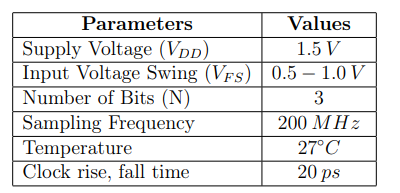
\includegraphics[width=1\linewidth]{spec.png}
    \caption{Specifications of SAR ADC}
    \label{fig:enter-label}
\end{figure}
\subsection{Comparator + RS Latch}
In this section, you need to design a latched comparator for the fine ADC. The Report the design procedure followed and tabulates the initial and final dimensions of all the transistors. Ensure that the comparator’s outputs are settling within a half-clock cycle.
\begin{figure}[H]
    \centering
    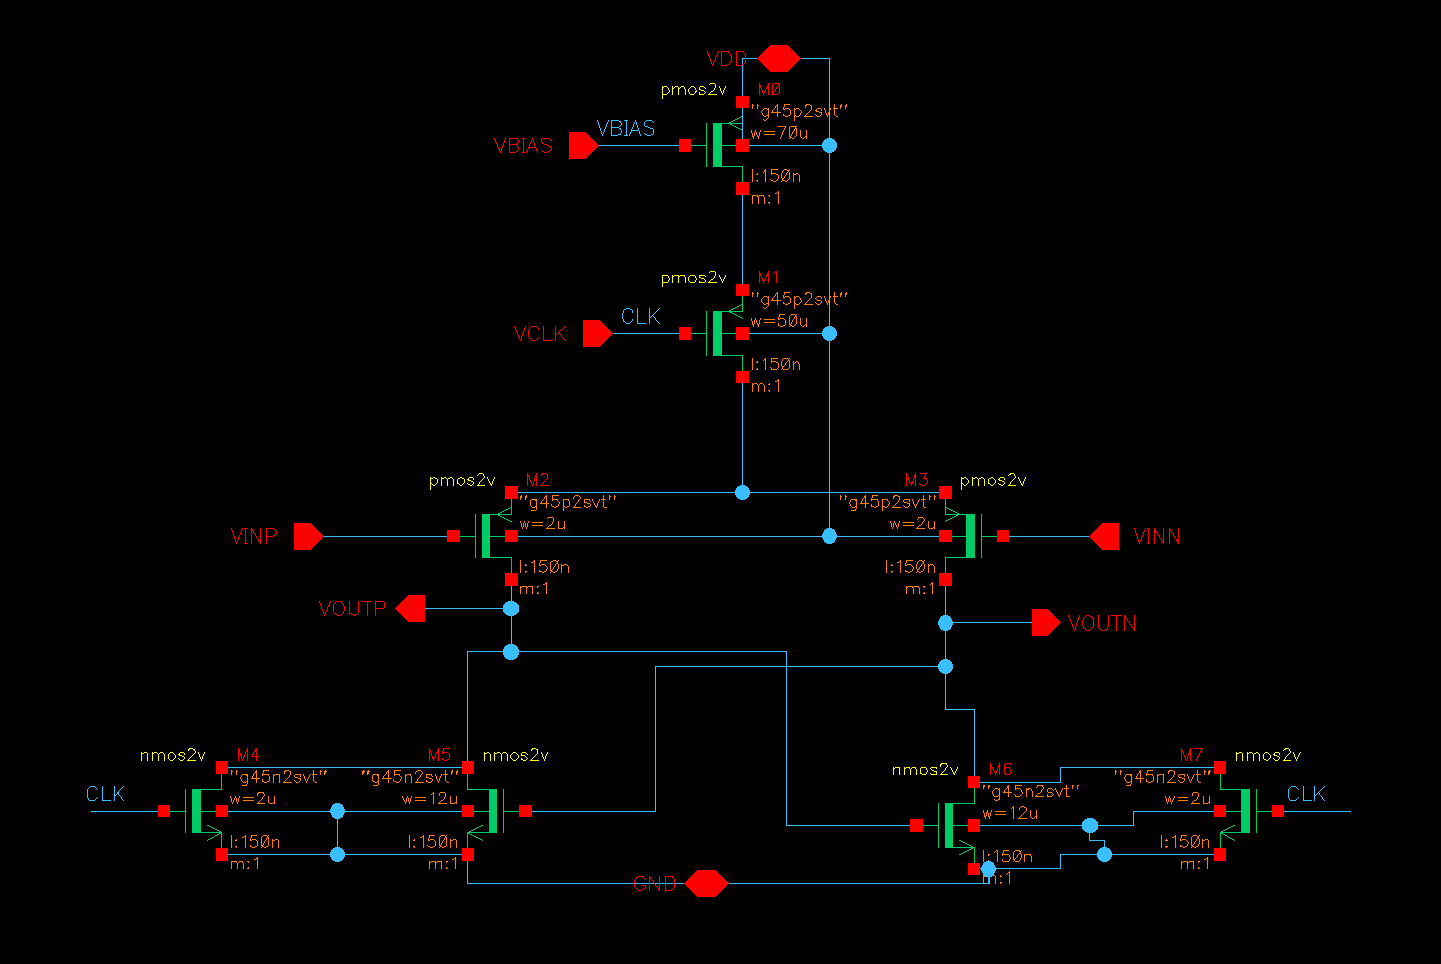
\includegraphics[max width = \textwidth]{3/3_sch_strongarm.png}
    \caption{PMOS Strong Arm Latch Comparator Schematic}
    \label{fig:enter-label}
\end{figure}

\begin{table}[H]
    \centering
    \begin{tabular}{|c|c|c|c|c|c|c|c|c|}
    \hline
        Design Variable & $M_1$ & $M_2$ & $M_3$ & $M_4$ & $M_5$ & $M_6$ & $M_7$ & $M_8$ \\
        \hline
        Width & 70u & 50u & 2u & 2u & 2u & 12u & 12u & 2u\\
        \hline
        Length & 150n & 150n & 150n & 150n & 150n & 150n & 150n & 150n\\
        \hline
    \end{tabular}
    \caption{Final parameter summary of PMOS Strong ARM latch comparator}
    \label{tab:my_label}
\end{table}

\begin{figure}[H]
    \centering
    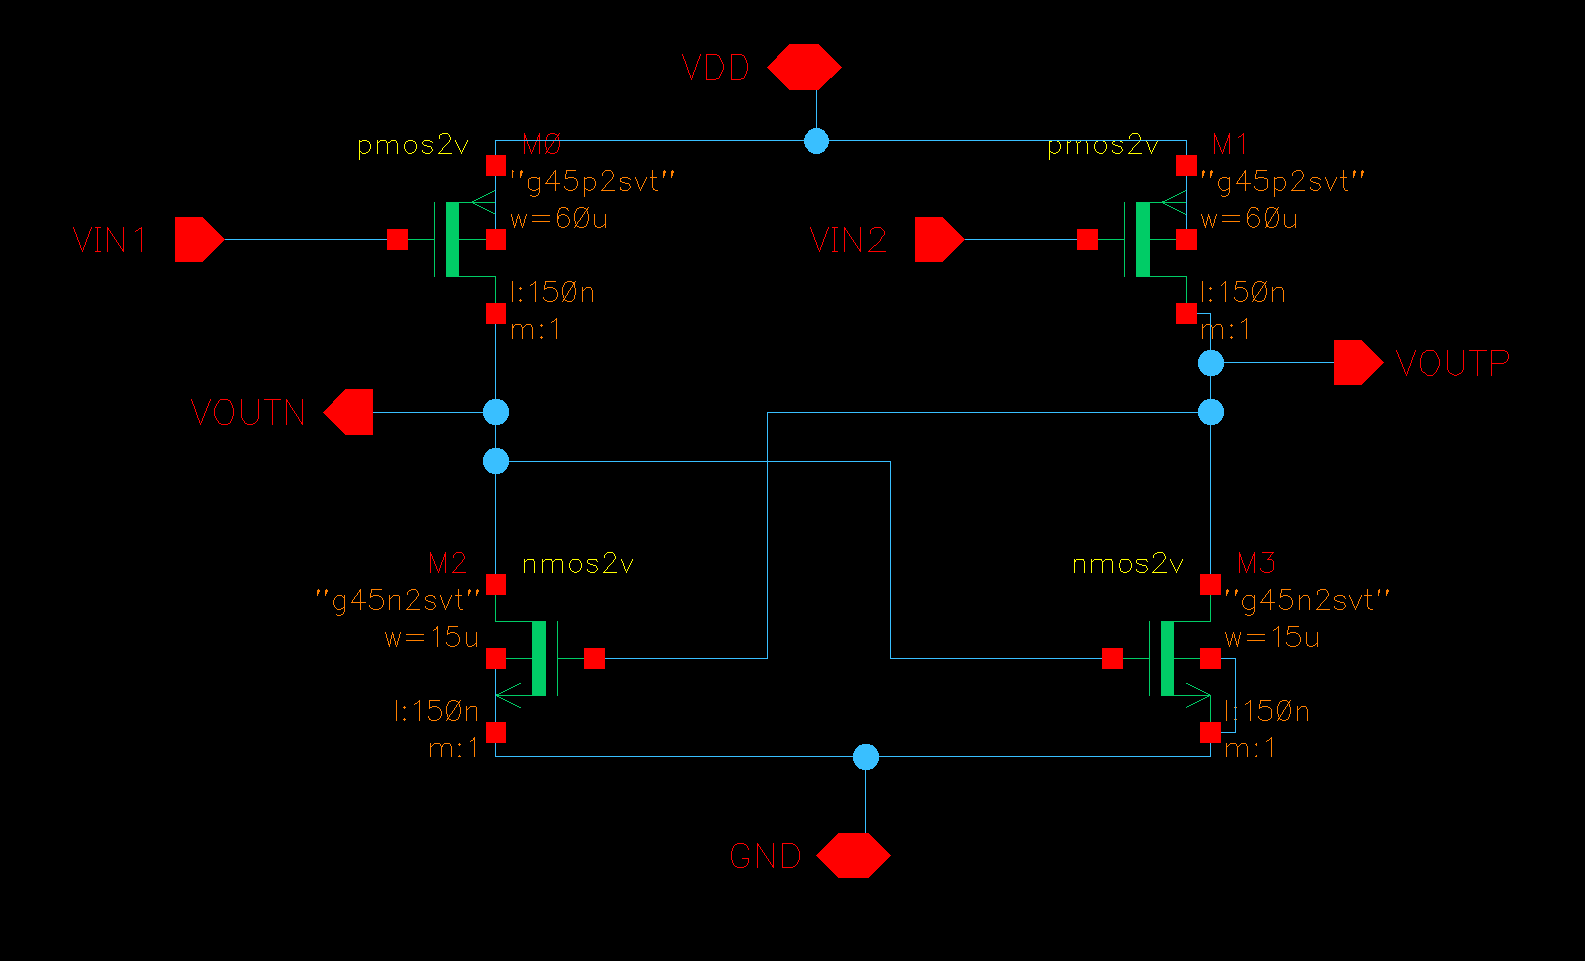
\includegraphics[max width = \textwidth]{3/3_sch_rslatch.png}
    \caption{RS Latch Schematic}
    \label{fig:enter-label}
\end{figure}

\begin{figure}[H]
    \centering
    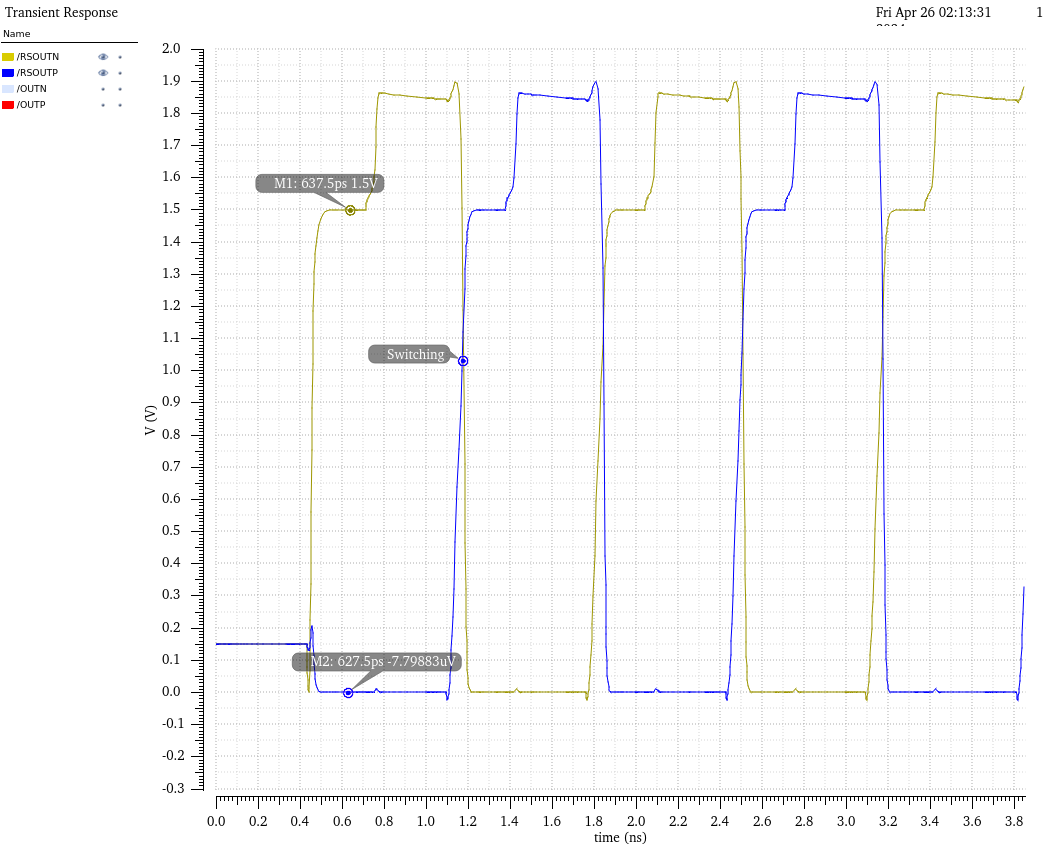
\includegraphics[max width = \textwidth]{3/3_RSOUT.png}
    \caption{RS Latch output waveform}
    \label{fig:enter-label}
\end{figure}

\begin{table}[H]
        \centering
        \begin{tabular}{|c|c|c|c|}
        \hline
         Design Variable & $M_{P1}$ & $M_{N1}$ & $M_{P2}$ & $M_{N2}$ \\
         \hline
         Width & 60u & 15u & 60u & 15u\\          
         \hline
         Length & 150n & 150n & 150n & 150n\\
         \hline
        \end{tabular}
        \caption{Final parameters for Preamplifier}
        \label{tab:my_label}
    \end{table}

\subsection{Binary weighted charge redistribution capacitive DAC}

\begin{itemize}
    \item[1.] Choose an appropriate unit capacitance value for the C-DAC considering the SNR requirements.
Justify the capacitance value chosen in the report.\\
SNR of the Sampler-ADC cascade is,
\begin{equation}
    SNR = \frac{\frac{A^2}{2}}{\frac{\Delta^2}{2}+\frac{KT}{C_1}}
\end{equation}

\noindent Ideal SNR = 56 dB = 10 log$\left( \frac{\frac{A^2}{2}}{\frac{\Delta^2}{2}}\right)$ $\implies$ $\frac{\Delta^2}{A^2}$ = $10^{-6.2}$

\noindent Degraded SNR = 56 - 2 = 54 dB.

\begin{equation}
    SNR = 54dB = 10\times log\left(  \frac{\frac{A^2}{2}}{\frac{\Delta^2}{2}+\frac{KT}{C_1}} \right)
\end{equation}

\begin{equation}
    C_1 = 90 \times 10^{-15}
\end{equation}


Since the SAR ADC is fully differential, the capacitance C1 would be twice C1. Therefore, C1 = 180 fF.
\noindent We took \textbf{$C_1$ = 217 fF}.

\item[2.] To introduce nonideality in the capacitor values, use the MATLAB script provided to generate the
values of the 5 capacitances to be used. You need to input your group number and the chosen value of the unit capacitance. Use the same capacitances for C-DACs on both sides of SAR ADC (e.g. C1p = C1n).\\
We had assumed the mean value of unit capacitance to be 7 fF and our group number is 5. The corresponding capacitance values(in fF) are 6.9760, 14.2333, 27.7853, 57.4759, and  111.9812.
\end{itemize}

\subsection{SAR Logic}

\begin{figure}[H]
    \centering
    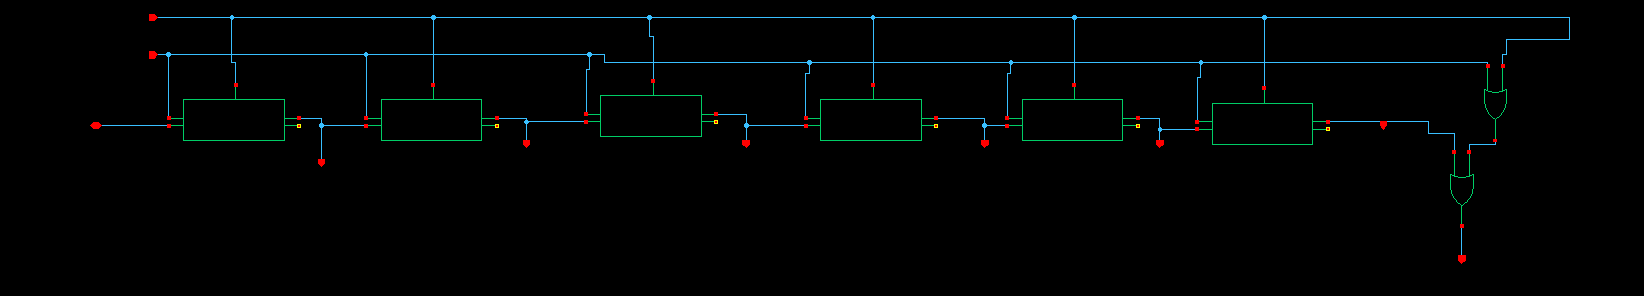
\includegraphics[max width = \textwidth]{3/3_sch_sarlogic.png}
    \caption{SAR Logic Schematic}
    \label{fig:enter-label}
\end{figure}


\begin{figure}[H]
    \centering
    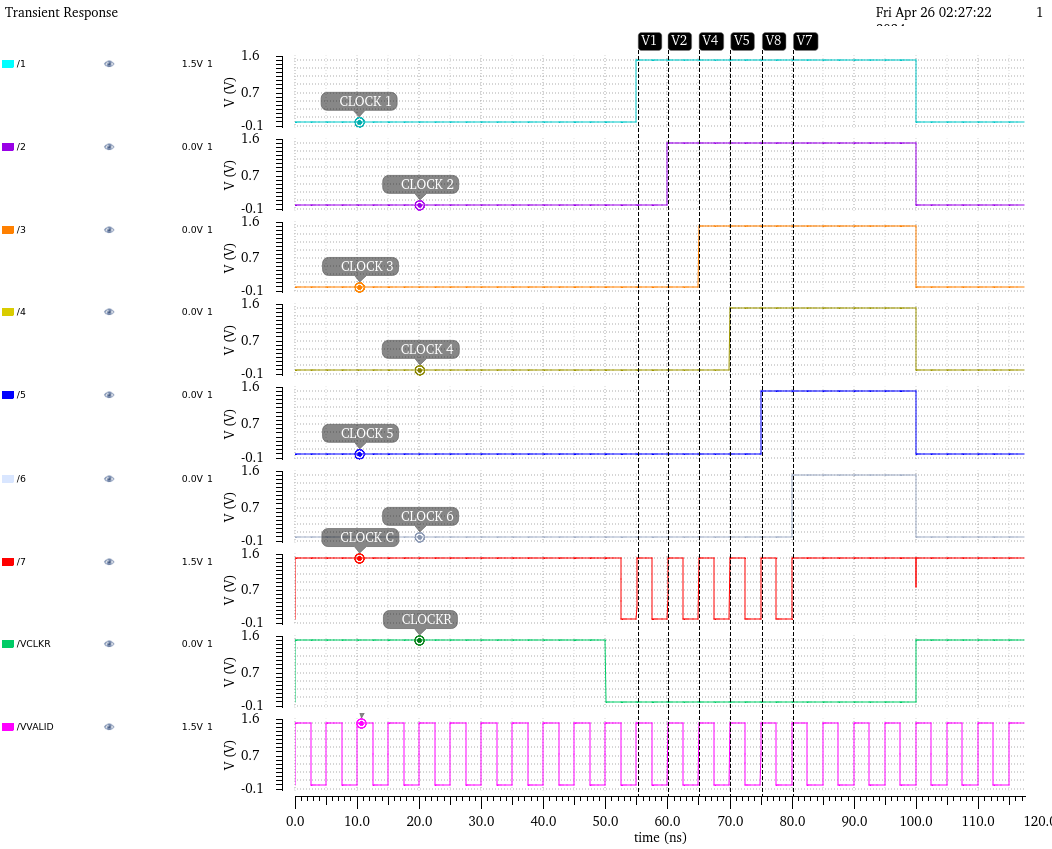
\includegraphics[max width = \textwidth]{3/3_SAR_LOGIC.png}
    \caption{SAR Logic}
    \label{fig:enter-label}
\end{figure}

\begin{figure}[H]
    \centering
    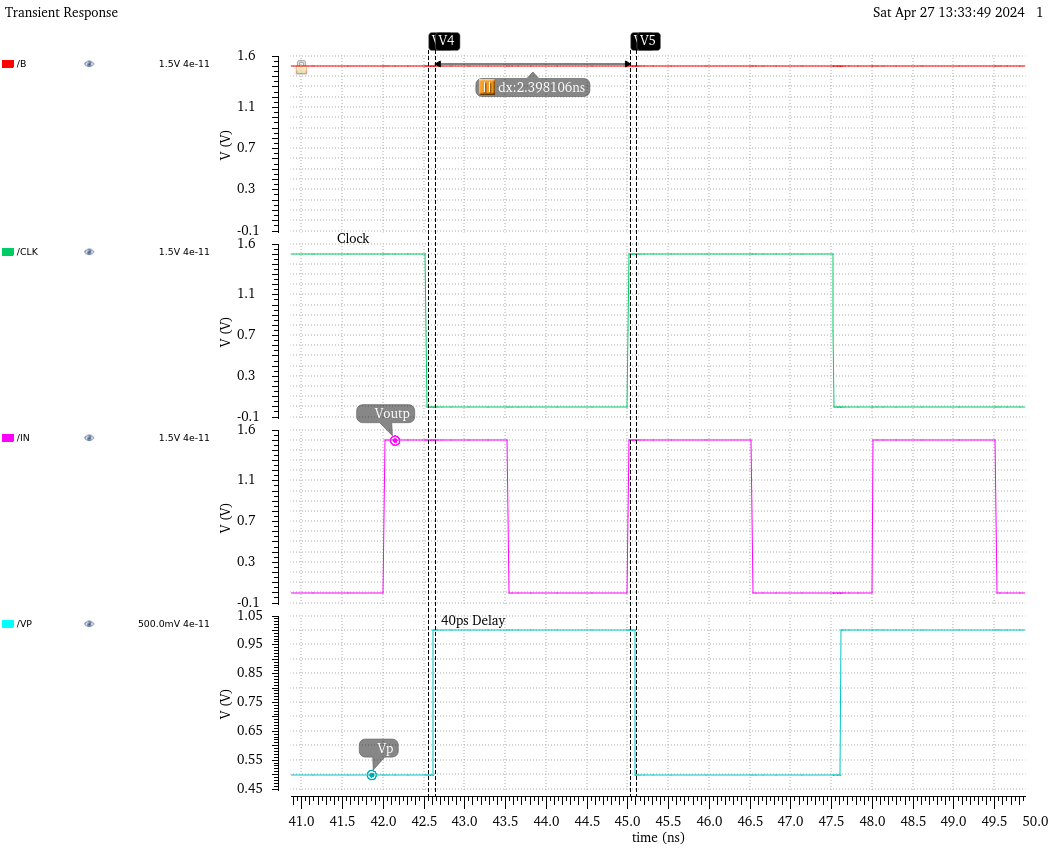
\includegraphics[max width = \textwidth]{3/3_CNTRL_LOGIC_C.png}
    \caption{SAR Logic}
    \label{fig:enter-label}
\end{figure}

\begin{figure}[H]
    \centering
    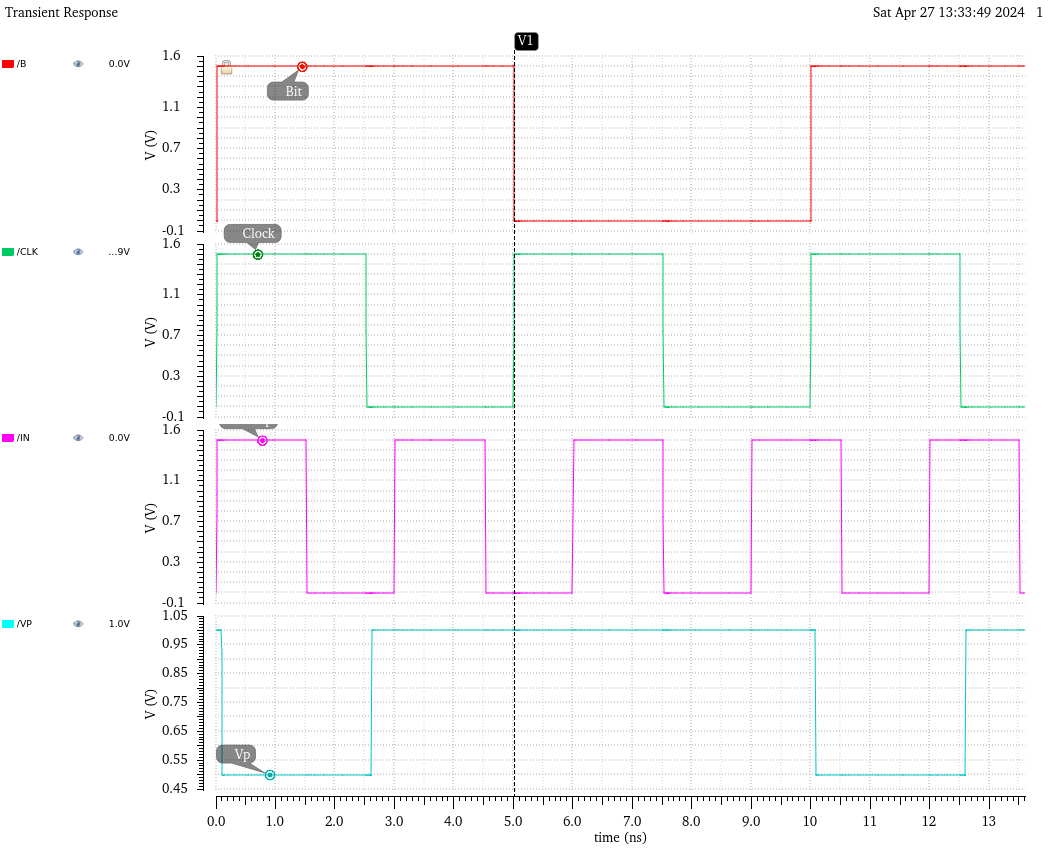
\includegraphics[max width = \textwidth]{3/3_CNTRL_LOGIC_NC.png}
    \caption{SAR Logic}
    \label{fig:enter-label}
\end{figure}

\begin{itemize}
    \item[(a)]\textbf{Monotonic Switching:}\\
    Plot the waveforms of Vinp and Vinn (inputs to the comparator of SAR ADC), showing the reduction in range due to the monotonic switching scheme for the complete SAR conversion cycle (6 clock cycles), for inputs - 0.64V ($V_{inp}$) and 0.72V ($V_{inn}$).

    \begin{figure}[H]
        \centering
        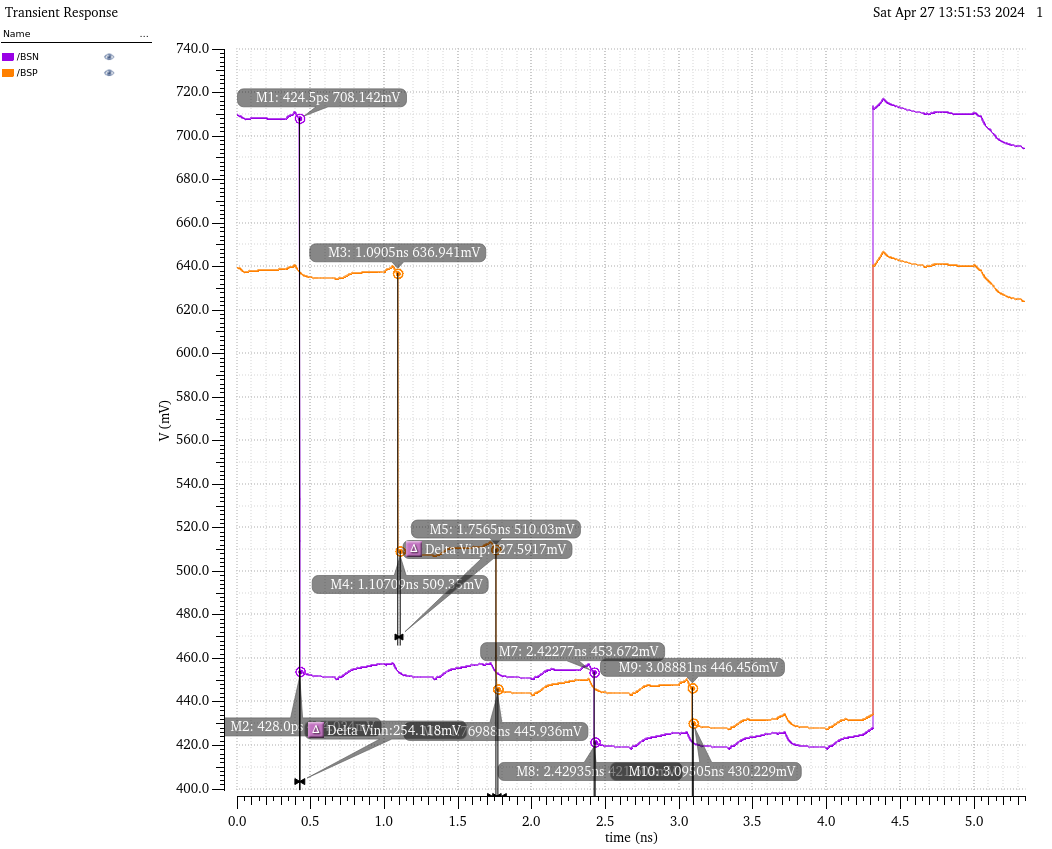
\includegraphics[max width = \textwidth]{3/3_VIN_MONOTONIC.png}
        \caption{Input waveform monotonic switching}
        \label{fig:enter-label}
    \end{figure}

    
    \begin{figure}[H]
        \centering
        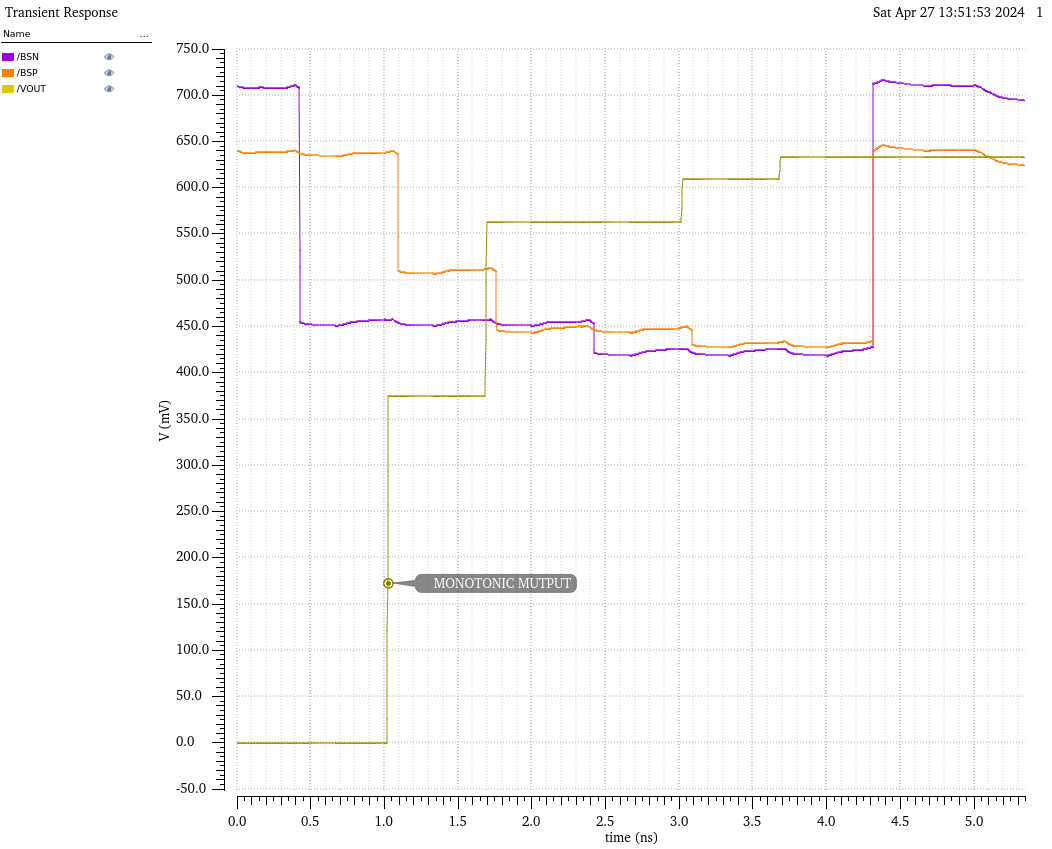
\includegraphics[max width = \textwidth]{3/3_VOUT_MONOTONIC.png}
        \caption{Output waveform monotonic switching}
        \label{fig:enter-label}
    \end{figure}

    

    \item[(b)] \textbf{Output waveform:}\\
    Use the provided ideal 6-bit DAC at the outputs of the SAR ADC. Apply a
differential input ramp as shown in Fig. 6 (b)for 800 clock cycles. Plot Output (after DAC) versus Input (differential ramp) characteristics of the ADC.
    \begin{figure}[H]
        \centering
        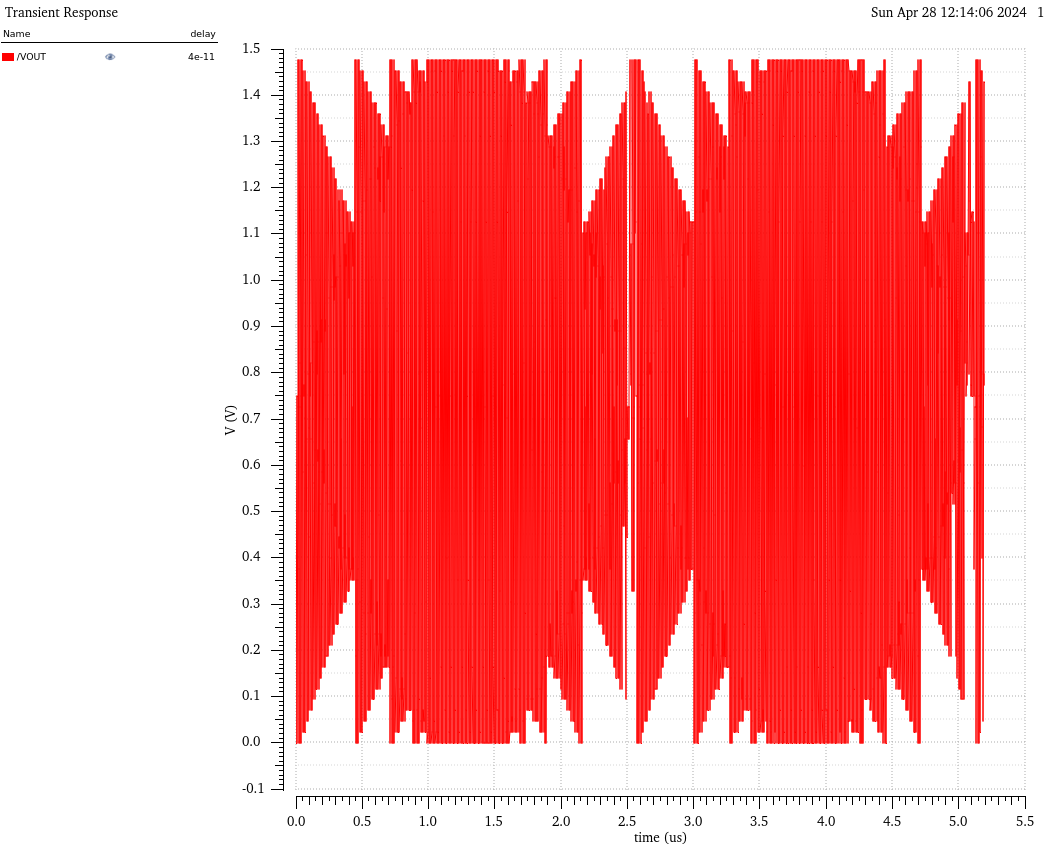
\includegraphics[max width = \textwidth]{3/3_DAC_VOUT.png}
        \caption{DAC output waveform characteristics of SAR ADC}
        \label{fig:enter-label}
    \end{figure}

    \item[(c)] \textbf{INL & DNL}
    Using the same applied inputs in part (b), for the obtained output characteristics, plot the INL and DNL of the ADC versus code using the MATLAB code provided.
    \begin{figure}[H]
        \centering
        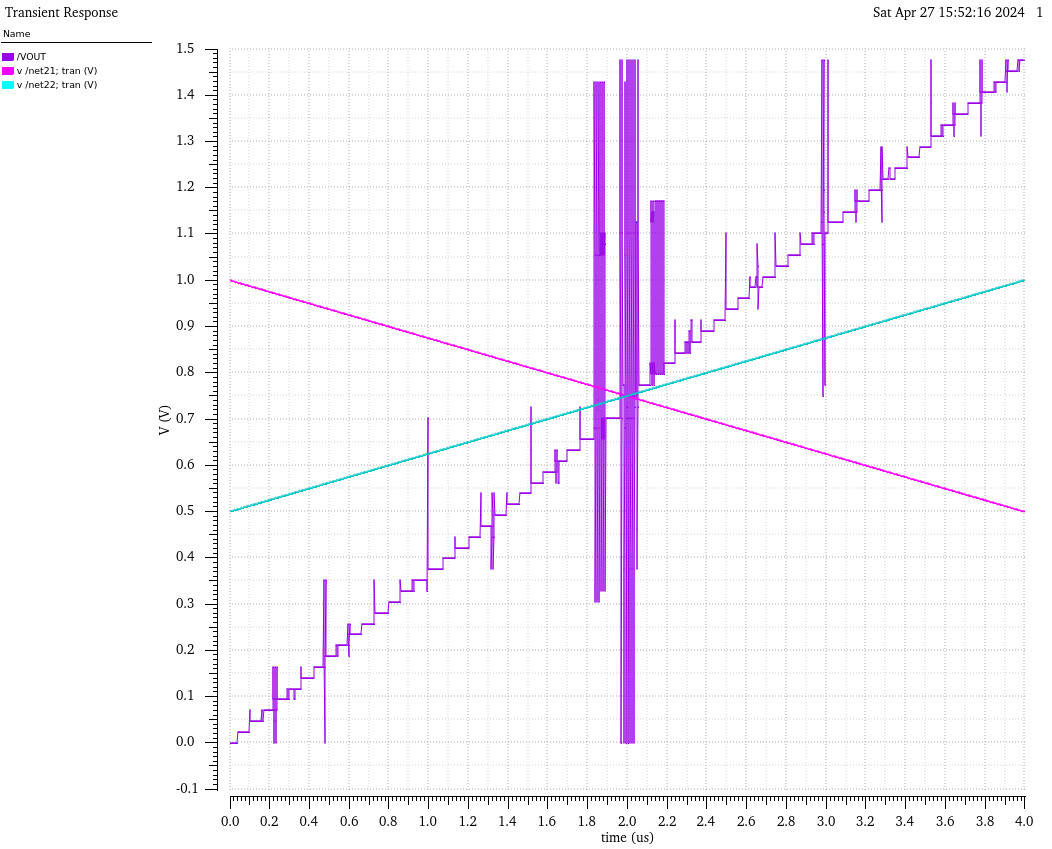
\includegraphics[max width = \textwidth]{3/3_VOUT_RAMP.png}
        \caption{Output characteristics of Ramp input}
        \label{fig:enter-label}
    \end{figure}

        \begin{figure}[H]
        \centering
        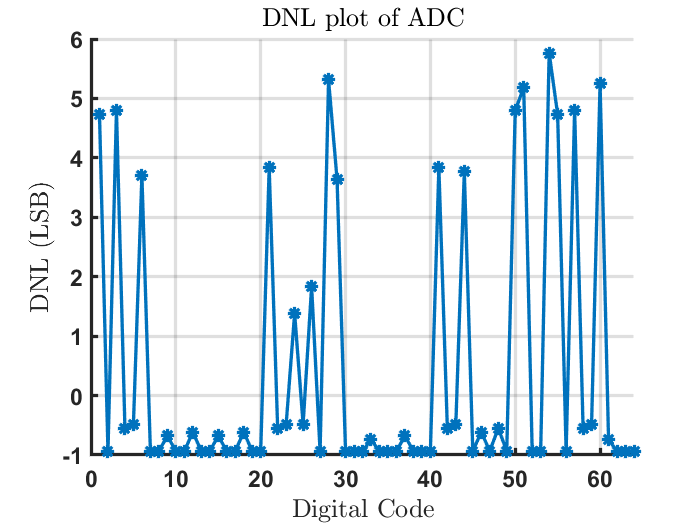
\includegraphics[max width = \textwidth]{3/DNL_SAR.png}
        \caption{DNL plot of SAR ADC}
        \label{fig:enter-label}
    \end{figure}

        \begin{figure}[H]
        \centering
        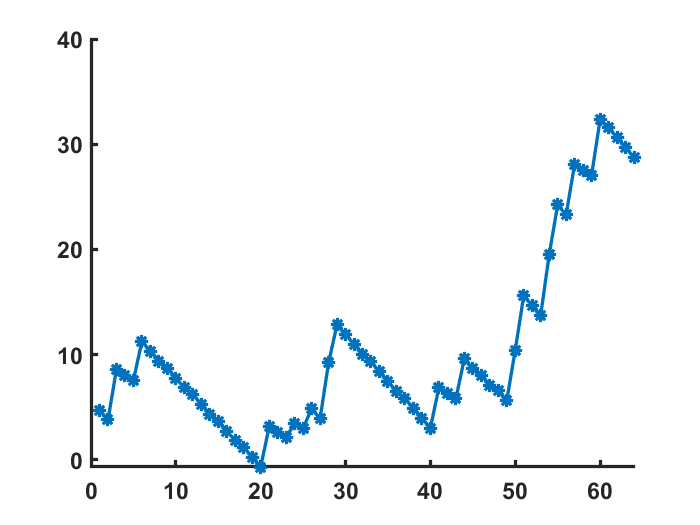
\includegraphics[max width = \textwidth]{3/3_INL.png}
        \caption{INL plot of SAR ADC}
        \label{fig:enter-label}
    \end{figure}

    \item[(d)] \textbf{FFT, SNR & ENOB:}
    To the circuit shown in Fig. 11, apply Vin1 = 0.75+0.25 Sin(2πfint) and Vin2 = 0.75−0.25 Sin(2πfint) with fin = m · fs/N, m = 511, N = 1024 and plot FFT of the Vout. Annotate the fundamental, 2nd and 3rd harmonic components and calculate ENOB, SNR.
    \begin{figure}[H]
        \centering
        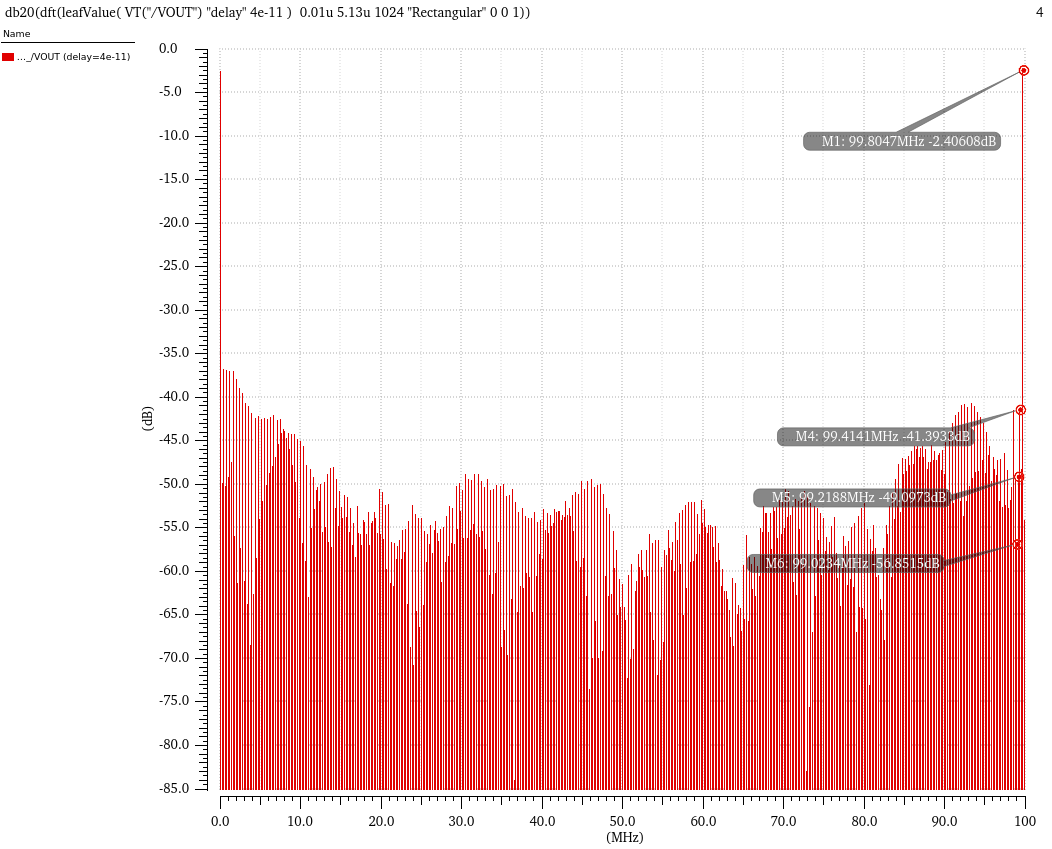
\includegraphics[max width = \textwidth]{3/3_FFT.png}
        \caption{FFT of output waveform for SAR ADC}
        \label{fig:enter-label}
    \end{figure}

    \begin{figure}[H]
        \centering
        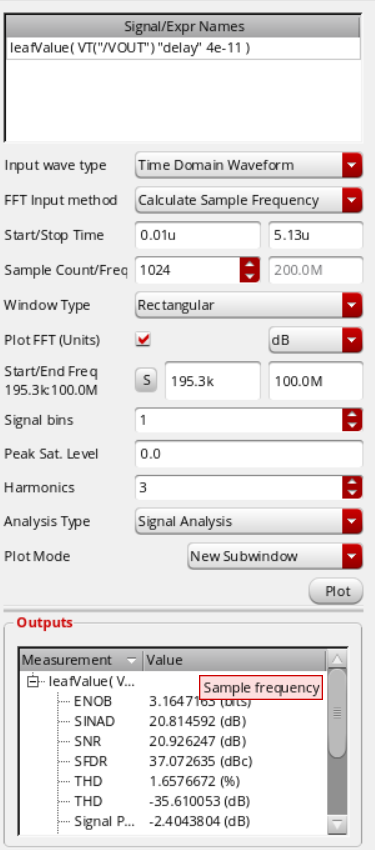
\includegraphics[max width = \textwidth]{3_ENOB_SNR.png}
        \caption{FFT of output waveform for SAR ADC}
        \label{fig:enter-label}
    \end{figure}

    \begin{figure}[H]
        \centering
        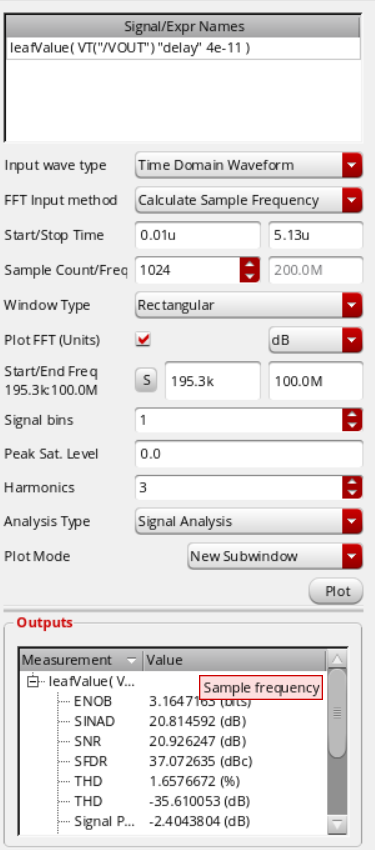
\includegraphics[max width = \textwidth]{3_ENOB_SNR.png}
        \caption{FFT of output waveform for SAR ADC}
        \label{fig:enter-label}
    \end{figure}
\end{itemize}




\end{document}